\documentclass[french]{article}
\usepackage{babel}
\usepackage[a4paper, total={6in, 10in}]{geometry}
\usepackage{rotating, graphicx}
\usepackage{listings}
\usepackage{color}
\usepackage{pdfpages}
\usepackage{caption}
\usepackage[toc]{appendix}
\usepackage{pdflscape}

\usepackage[svgnames]{xcolor} % Required for colour specification
\usepackage[utf8]{inputenc} % Required for inputting international characters
\usepackage[T1]{fontenc} % Output font encoding for international characters
\usepackage{fouriernc} % Use the New Century Schoolbook font

\DeclareGraphicsExtensions{.pdf,.png,.jpg}
% listings color configuration to display beautifuuul code
\definecolor{Monokaigreen}{rgb}{0.42,0.72,0.18}
\definecolor{Monokaimagenta}{rgb}{0.86,0.08,0.24}
\definecolor{Monokaiblue}{rgb}{0.40,0.85,0.94}
\definecolor{Monokaibg}{rgb}{0.15,0.16,0.13}
\definecolor{splashedwhite}{rgb}{1.0, 0.99, 1.0}
\definecolor{richelectricblue}{rgb}{0.03, 0.57, 0.82}
\definecolor{pinegreen}{rgb}{0.0, 0.47, 0.44}
\definecolor{ivory}{rgb}{1.0, 1.0, 0.94}
\definecolor{ghostwhite}{rgb}{0.97, 0.97, 1.0}
\definecolor{floralwhite}{rgb}{1.0, 0.98, 0.94}
\definecolor{gray}{rgb}{0.5,0.5,0.5}

 
\definecolor{codegreen}{rgb}{0,0.6,0}
\definecolor{codegray}{rgb}{0.5,0.5,0.5}
\definecolor{codepurple}{rgb}{0.58,0,0.82}
\definecolor{backcolour}{rgb}{0.95,0.95,0.92}

\lstdefinestyle{code_style}{
    backgroundcolor=\color{backcolour},   
    commentstyle=\color{codegreen},
    keywordstyle=\color{magenta},
    numberstyle=\tiny\color{codegray},
    stringstyle=\color{codepurple},
    basicstyle=\footnotesize,
    breakatwhitespace=false,         
    breaklines=true,                 
    captionpos=b,                    
    keepspaces=true,                 
    numbers=left,                    
    numbersep=4pt,                  
    showspaces=false,                
    showstringspaces=false,
    showtabs=false,                  
    tabsize=2
}

\lstset{style=code_style}
 

\makeatletter
%same as \subsubsection but level 4
\renewcommand\paragraph{\@startsection{paragraph}{4}{\z@}%
                                     {-3.25ex\@plus -1ex \@minus -.2ex}%
                                     {1.5ex \@plus .2ex}%
                                     {\normalfont\normalsize\bfseries}}
% number \paragraph
\setcounter{secnumdepth}{4}

\lstset{frame=shadowbox,
	language=Java,
	aboveskip=3mm,
	belowskip=3mm,
	showstringspaces=false,
	columns=flexible,
	basicstyle={\small\ttfamily},
	numbers=left,
	numberstyle=\tiny\color{gray},
	keywordstyle=\color{Monokaibg}\bfseries,
	commentstyle=\color{pinegreen},
	stringstyle=\color{Monokaigreen},
	breaklines=true,
	breakatwhitespace=false,
	tabsize=3,
	captionpos=b,                    % sets the caption-position to bottom
	frame=single,
	rulecolor=\color{gray},
}

\title{Sections and Chapitres}
\author{Quentin Gigon}
\date{ }

\begin{document}

\begin{titlepage} % Suppresses headers and footers on the title page
	
	\centering % Centre everything on the title page
	
	%------------------------------------------------
	%	Top rules
	%------------------------------------------------
	
	\rule{\textwidth}{1pt} % Thick horizontal rule
	
	\vspace{2pt}\vspace{-\baselineskip} % Whitespace between rules
	
	\rule{\textwidth}{0.4pt} % Thin horizontal rule
	
	\vspace{0.1\textheight} % Whitespace between the top rules and title
	
	%------------------------------------------------
	%	Title
	%------------------------------------------------
	
	\textcolor{Red}{ % Red font color
		{\Huge Travail de Bachelor}\\[0.5\baselineskip] % Title line 1
	}

	\textsc{\LARGE Diffusion de flux d'information sur les écrans de la HEIG-VD}\\[1.5cm] % Publisher

	
	\vspace{0.025\textheight} % Whitespace between the title and short horizontal rule
	
	\rule{0.3\textwidth}{0.4pt} % Short horizontal rule under the title
	
	\vspace{0.1\textheight} % Whitespace between the thin horizontal rule and the author name
	
	%------------------------------------------------
	%	Author
	%------------------------------------------------
	
\begin{minipage}{0.4\textwidth}
\begin{flushleft} \large
\emph{Author:}\\
Quentin \textsc{Gigon} % Your name
\end{flushleft}
\end{minipage}
~
\begin{minipage}{0.4\textwidth}
\begin{flushright} \large
\emph{Supervisor:} \\
Pr. Pier \textsc{Donini}\\
Mr. Jérôme \textsc{Varani}
% Supervisor's Name
\end{flushright}
\end{minipage}\\[2cm]
	
	\vfill % Whitespace between the author name and publisher
	
	%------------------------------------------------
	%	Publisher
	%------------------------------------------------
	
	\textsc{\LARGE Haute Ecole d'Ingénierie et de Gestion du Canton de Vaud}\\[1.5cm] % Publisher
	\textsc{\large Département des Technologies d'Information et de Communication}\\[0.5cm] % Minor heading such as course title

	
	\vspace{0.1\textheight} % Whitespace under the publisher text
	
	%------------------------------------------------
	%	Bottom rules
	%------------------------------------------------
	
	\rule{\textwidth}{0.4pt} % Thin horizontal rule
	
	\vspace{2pt}\vspace{-\baselineskip} % Whitespace between rules
	
	\rule{\textwidth}{1pt} % Thick horizontal rule
	
\end{titlepage}

\maketitle

\tableofcontents
\newpage
\listoffigures
\newpage
\lstlistoflistings

\newpage

\section{Préface}

Dans ce document seront utilisés des termes anglais avec une majuscule. Ces termes représentent des objets ou entités de l'application associés à des éléments du monde réel. Leur traduction française étant souvent moins représentative, le choix a été fait de les utiliser tels quels. Ces termes sont les suivants :
\begin{itemize}
	\item Team
	\item Schedule
	\item Diffuser
\end{itemize}
Certains termes informatiques n'ayant pas de réelle traduction mot-à-mot peuvent également avoir été utilisés.


\newpage

\section{Introduction au projet}

La HEIG-VD dispose de nombreux écrans pour la diffusion d'informations, répartis sur ses différents sites. A l'heure actuelle, un système existe déjà pour permettre une certaine organisation du contenu diffusé mais il s'agit plutôt d'une solution temporaire. Il ne fournit en effet que des fonctionnalités de diffusions pures, ne propose pas de système d'utilisateurs ou d'équipes et ne propose pas de modèle générique pour l'ajout de flux au sein de l'application. \newline
Le but de ce travail de Bachelor est donc de centraliser la gestion des écrans et de l'affichage de flux à travers une application Web, et de fournir un programme répondant le plus possible aux exigences fournies. Si ces dernières sont explicitées dans le cahier des charges (voir Annexe A), en voici une courte liste non-exhaustive:
\begin{itemize}
	\item Gérer les droits des utilisateurs
	\item Permettre des opérations de maintenance à distance
	\item Limiter l'affichage de flux selon diverses conditions
	\item Gérer l'ajout d'écrans au système 
	\item Modélisation d'un flux de données \newline
\end{itemize}

Un élément très important dans la direction qu'a prise le projet est la différence matérielle entre les écrans. Il s'agit en effet soit de SmartTV, soit de PC faisant tourner Ubuntu Server. Cela a eu un gros impact dans la construction de l'architecture du programme, car il fallait une solution de rendu sur les écrans compatibles avec les deux types de matériel. La technique utilisée actuellement, soit un affichage des flux dans l'onglet d'un navigateur, a été très vite définie comme la solution à implémenter.


\newpage
\section{Présentation des technologies utilisées}

\subsection{Framework Play!}
Play! est un framework web open-source qui suit le modèle MVC et qui permet d'écrire rapidement des applications web en Java (ou en Scala). A la différence d'autre frameworks Java, Play! est \textit{stateless}, ce qui veut dire qu'il n'y a pas de session créée à chaque connexion. 


\subsection{EventSource}
Les EventSource, ou Server-Sent Events (SSE), sont une technologie permettant à un navigateur internet de recevoir des mises à jour automatiques d'un serveur par une connexion HTTP persistante. L'API Javascript (\textit{Server-Sent Events EventSource API}) fut instaurée la première fois dans Opera en 2006 et a été normalisée dans le cadre de HTML5. \par
Les Events envoyés sont au format \textit{text/event-stream} et sont reçus par le navigateur sous la forme d'Event de type \textit{message} La connexion reste ouverte tant qu'elle n'a pas été fermée par le navigateur, et contrairement aux WebSockets, les SSE sont uni-directionnels et ne permettent donc pas aux clients de communiquer avec le serveur. 

\subsection{PostgreSQL}
PostgreSQL est un système de gestion de base de données relationnelle et open-source. Les différence principales entre PostgreSQL et ses concurrents sont la prise en charge de plus de types de donnée que les types traditionnels (entiers, caractères, ...), ainsi qu'une communauté plus active et un développement plus rapide que MySql par exemple.

\subsection{JPA}
La Java Persistence API (JPA) est une interface de programmation permettant aux utilisateurs de la plateforme Java (SE et EE) d'organiser facilement et clairement leurs données relationnelles. Elle utilise des annotations pour définir des "objet-métiers" qui serviront d'interface entre la base de données et l'application. \newline
JPA définit aussi le Java Persistence Query Language (JPQL), qui est utilisé pour créer les requêtes SQL dans le cadre de JPA. Les requêtes effectuées dans ce langage ressemblent beaucoup à du SQL classique, sauf que le JPQL fonctionne avec des entités (créées avec des annotations) plutôt que des tables de la base de données.

\subsection{HTML5}
HTML5 est la dernière version majeure du HTML (octobre 2014). Elle vient avec plein de nouveaux éléments, comme la balise \textit{video}, qui permet d'insérer un contenu vidéo en streaming dans un fichier HTML, ou encore \textit{footer}, qui lui permet de facilement afficher du texte en bas de page.

\subsection{Quartz}
Quartz est un framework open-source offrant des moyens de "scheduling" pouvant être intégré à n'importe quel projet Java. Il permet de créer des "schedules" pouvant effectuer jusqu'à des milliers de jobs. Ces jobs sont des composants Java standards et peuvent donc effectuer à peu prêt n'importe quelle tâche. Il est utilisé dans le cadre du projet pour construire des horaires de flux et générer des événements.

\newpage
\section{Analyse et Architecture}

Dans les chapitres suivants seront détaillés l'architecture du programme (les modèles et leur représentation réelle) ainsi que les différentes idées et versions qui ont été envisagées. Leurs équivalents en base de données seront explicités dans le chapitre suivant.

\subsection{Site}
Un Site représente un emplacement physique de l'HEIG-VD, donc les sites de Cheseaux, St-Roch et Y-Park. Ils servent principalement à localiser les écrans et restreindre l'affichage de flux selon le lieu. Par exemple pour l'affichage des horaires, où l'horaire de Cheseaux importe peu les gens de St-Roch et vice-versa.\newline
 Une idée et demande de mon mentor était d'avoir un seul flux horaire qui, selon le site où il est affiché, prend un paramètre de requête différent (p.ex. \textit{www.horaire.ch?site=che}). Cela permet d'offrir plus de possibilités lors la création de flux pour l'utilisateur. Malheureusement, à cause d'un oubli de ma part, cette fonctionnalité n'est pas présente et il faut donc avoir un flux d'horaire pour chaque site.
 
\subsection{Team et utilisateurs}
Pendant la phase d'analyse, il a été spécifié qu'un système d'équipe était nécessaire, afin de restreindre les fonctions du programme selon l'appartenance de l'utilisateur courant à telle ou telle équipe. Cela faisait également sens vu que le programme sera utilisé par les différents départements de la HEIG-VD.\newline
Les \textbf{Teams} ont donc une place centrale dans l'architecture du programme car les actions proposées à l'utilisateur utilisent uniquement les données accessibles par son équipe. Elle est composée de membres et de chefs d'équipe, qui sont les deux représentés par des \textbf{TeamMember}, et qui ont différents niveaux d'accès. \newline
Dans la première version proposée pour la représentations des utilisateurs, les équipes étaient composées de trois types : un administrateur, des chefs d'équipe et des membres. Lors de la rédaction des cas d'utilisation et après un entretien avec mon mentor, il a été décidé que d'avoir autant de status différents au sein d'une même équipe rendait la division des actions possibles moins logique et l'utilisation finale plus compliquée sans grandes raisons. Les administrateurs d'équipe ont ainsi disparu pour être remplacés par les chefs d'équipe.\newline
En plus des équipes, il fallait également un rôle d'administrateur central, à qui sont réservées quelques fonctionnalités (p.ex. l'ajout de nouveaux écrans au système).

\subsection{Organisation des flux}

Un flux dans ce programme représente un contenu à afficher sur un écran. Pendant la phase d'analyse, il a été spécifié que l'application devait pouvoir gérer deux sortes de flux: un flux externe à l'application comme le flux de la RTS ou un flux interne, comme les horaires des cours ou les réservations de salle. \newline

J'avais également proposé de fournir un template RSS permettant un ajout facile de nouveau flux RSS, mais cette fonctionnalité à été abandonnée par manque de temps.

En ce qui concerne leur diffusion, il fallait proposer un moyen d'organiser un horaire de flux ainsi que la possibilité d'envoyer immédiatement un flux sur un écran. Deux types d'objets ont ainsi été créés : des Schedules, qui représentent l'horaire des flux pour une journée et des Diffusers, qui eux permettent d'envoyer un flux aux écrans sans forcement passer par un Schedule. Ils sont explicités dans les sections suivantes.

\subsubsection{Flux}

Un flux est caractérisé par un nom, un type, une durée d'affichage et un contenu. Ce contenu est défini par le type du flux; un flux 'URL' contiendra une url, tandis un flux de type 'Image' contiendra l'adresse de l'image sur le serveur.

Ils sont regroupés en quatre types:
\begin{itemize}
	\item URL, ou type standard
	\item Vidéo
	\item Image
	\item Texte
\end{itemize}
Le traitement de ces flux par le système et la manière par laquelle ils sont affichés sur les écrans changent selon leur type. Par exemple, un flux 'Image' sera rendu dans une balise <img>, tandis qu'un flux 'URL' le sera dans une \textit{iframe}.

De plus, il y a trois sortes de flux: des flux généraux, des flux localisés et des flux de fallback. Ils sont comme des sous-populations de flux: ils possèdent une référence vers un flux existant. \newline
Comme son nom l'indique, un flux général peut être diffusé partout. Par opposition, un flux localisé est lui uniquement affichable sur le Site correspondant.
Et enfin un flux peut être un flux de fallback. Ces flux sont spécifiés à la création d'un Schedule et utilisés par celui-ci pour remplacer un flux programmé mais pour lequel le serveur ne détecte aucune données à afficher. Dans le cas où aucun flux de fallback n'est sélectionné, un flux d'erreur est envoyé à la place. \newline 

La durée d'affichage d'un flux est déterminée par deux facteurs : son nombre de phases et la durée d'une phase. Cette décomposition a été implémentée car elle règle un problème mentionné par mon mentor, à savoir qu'il y a des flux (les réservations de salles par exemple) qui peuvent avoir trop de données à afficher en une seule fois (30 éléments pour une table de 20, etc). \newline
Une autre demande de mon mentor était d'avoir un système permettant de vérifier si un flux avait l'autorisation de s'afficher selon diverses conditions, la plus simple étant une condition temporelle avec des bornes. Ma solution proposée est d'avoir un micro-serveur ou service à qui l'on peut faire des requêtes et qui, selon les paramètres de la requête, nous renvoie des fichiers Json contenant diverses informations. Pour reprendre l'exemple d'une condition temporelle, on peut imaginer que l'application doive vérifier si un flux à le droit de s'afficher. Elle fera donc une requête à ce service qui ressemblera à ceci: 
\begin{verbatim}
	https://flux_check.com?fluxId=4&type=time
\end{verbatim}
On recevrait alors un Json contenant une borne de début et une de fin et le programme pourrait vérifier si la date courante est dans les bornes ou non. On peut aussi imaginer d'autres type de vérification/limitation d'où le paramètre de requête \textit{type}.

\subsubsection{Schedules}
Un Schedule représente un horaire de flux. Un Schedule n'est pas assigné à des écrans à sa création mais au moment de son activation pour permettre  une réutilisation plus facile des Schedules créés. Chaque chef d'équipe peut en créer qui seront utilisables par tous les membres de son équipe. \newline

La première version de cet horaire modélisait un cycle, où les flux choisis par l'utilisateur bouclaient à l'infini. Ce système a été utilisé avec succès pour de la recherche et des tests sur la faisabilité du programme mais fut vite obsolète quand il s'agissait d'avoir plus de contrôle sur l'horaire, par exemple définir une heure de début pour un flux donné. \newline
Il a donc fallu inventer un système permettant à la fois de créer un horaire à respecter pour les Schedules et de modifier cet horaire à la volée pour les Diffusers, tout en garantissant la cohérence du programme. 
	\newline
Ma première idée fût de représenter une journée complète d'affichage par des blocs de 1 minute chacun. Cette version n'était pas satisfaisante car trop compliquée pour un résultat très moyen. \newline
La modélisation définitive des horaires est donc la suivante: \newline
Un horaire peut être composé de deux éléments différents: une boucle de flux (FluxLoop) et un flux programmé (FluxTrigger). Une boucle envoie ses flux les uns après les autres jusqu'à ce que ce soit à un flux programmé d'être envoyé. Ces éléments sont utilisés en coopération avec le framework Quartz afin de créer des CRON qui serviront de déclencheur pour l'envoi de Flux. 

Si on regarde maintenant la procédure de création puis d'activation d'un Schedule:
Quand un utilisateur crée un Schedule, il peut lui spécifier plusieurs choses:
\begin{itemize}
	\item Un nom (unique)
	\item Des flux avec heure de début (FluxTriggers)
	\item Des flux sans heure de début (FluxLoop)
	\item Des flux de fallback
\end{itemize}

Pour chaque flux avec une heure de début associée, une "entrée de calendrier", ou FluxTrigger, est créée et ajoutée dans la base de données. Cette "entrée" contient des références vers le Flux et le Schedule concernés, ainsi que son heure de départ (en heures:minutes).\newline
Chaque flux sans heure de début est regroupé avec les autres flux sans heure de début faisant partie du même ensemble (ces ensembles sont délimité par les flux possédant une heure de début) pour créer des FluxLoop et les ajouter à la base de données. Ces boucles contiennent des références vers le Schedule et les Flux concernés ainsi que leur heure de départ. Lors de discussions avec mon mentor, il avait été demandé que les FluxLoop n'aient pas d'heure de départ mais que celle-ci soit calculée sur le moment. Cela devait aussi permettre de réduire le nombre d'entrées de la table FluxLoop car on pouvait alors ne pas dupliquer des boucles référençant les mêmes flux mais dans un ordre différent. J'ai essayé de modifier le programme de cette manière mais je suis tombé face à un problème auquel je n'ai pas trouvé de solution efficace : comment savoir quel FluxLoop devait être démarré à quel moment. Les solutions que j'ai envisagé ne me convenait pas car elles scindaient la logique du programme en deux ou nécessitaient elles aussi des modifications de la table FluxLoop. \newline
Les flux de fallback sont ajoutés tels quels au Schedule.\newline

A l'activation d'un Schedule, on peut choisir parmi les écrans auxquels on a accès ceux qui seront concernés. Un objet RunningSchedule est créé, une entité temporaire qui existe uniquement tant que le Schedule reste actif. 
Ensuite, les objets créés précédemment (soit les FluxLoop et FluxTrigger) sont utilisés pour créer les CRON représentant les entrées du Schedule. La manière dont ces CRON sont créés est détaillée dans le chapitre \textbf{Réalisation}.\newline 
Ce système permet de répondre à une autre demande du projet, la reprise de l'exécution des Schedules actifs lors du redémarrage du serveur ou après une maintenance. On peut en effet facilement recréer tous les CRON d'un Schedule et reprendre l'exécution depuis l'heure courante.


\subsubsection{Diffuser}
Les Diffusers sont utilisés pour diffuser directement du contenu sur les écrans, sans devoir passer par un Schedule. Ils ont été rajoutés car mon application manquait d'un moyen d'envoyer rapidement un flux, p.ex. pour un message d'alerte. \newline
A sa création, l'utilisateur doit spécifier les attributs suivants:
\begin{itemize}
	\item Un nom (unique)
	\item Un flux
	\item Une heure de début
\end{itemize}

Le comportement d'un Diffuser est le suivant: il remplace l'exécution d'un potentiel Schedule actif pour les écrans auxquels il est associé tant qu'il est actif. Si un Diffuser est activé pour un écran n'ayant pas de Schedule actif, un CRON est créé pour pouvoir quand même envoyer le flux diffusé aux écrans. \newline
Comme pour les Schedules, un Diffuser actif est un RunningDiffuser, lui aussi une entité temporaire qui reste active selon la validité spécifiée à sa création ou jusqu'à sa désactivation/destruction. Une fois que le RunningDiffuser est arrivé en fin de vie, les écrans auxquels il diffusait un flux peuvent reprendre leur Schedule. 

\newpage
\subsection{Ecrans}

Lors de mes discussions avec mon mentor, il a été assez vite recommandé et conseillé que j'utilise des Eventsources (voir doc) pour envoyer les ordres d'affichages aux écrans. Les sections suivantes résument et décrivent leur utilisation dans ce programme.

\subsubsection{Affichage}
Pour l'affichage des flux sur les écrans, les technologies autorisées étaient le HTML5, CSS3 et Javascript pur (sans frameworks). La demande initiale était de pouvoir afficher le contenu associé à une URL grâce aux iframes. Il fallait donc un moyen pour les écrans de recevoir une URL sous forme texte. En partant de ce constat, j'ai remarqué que si un événement contenait une URL en texte, il pouvait contenir d'autres données. J'ai donc proposé d'implémenter des flux de types image et texte. \newline
Les écrans sont capable de déterminer le type du flux reçu et de l'afficher de la manière adéquate. Les différents moyens utilisés l'affichage en question sont décrits dans la section Réalisation.

\subsubsection{Evénements}
Un des problèmes à résoudre était la question d'envoyer les bons événements aux bons écrans.
 Il y avait deux manières principales de faire, soit envoyer tous les événements à tous les écrans avec la liste des écrans concernés, soit générer dynamiquement des endpoints pour chaque Schedule. Pour des raisons de simplicité et parce que le nombre d'écrans restera raisonnable, la première possibilité a été choisie. \newline
Les événements générés par les Schedules sont donc envoyés à tous les écrans s'étant connectés auprès du serveur. Chaque événement contient les adresses MAC des écrans concernés et c'est à l'écran de vérifier s'il est concerné par l'événement qu'il vient de recevoir.\newline
Un événement est construit de la manière suivante: il contient son type, ses "données" (url ou texte) et les écrans concernés. \newline
Ci-dessous un exemple pour chaque type:\newline


\begin{itemize}
	\item URL:\begin{verbatim}
					url?https://heig-vd.ch|mac_address1,mac_address2
			  \end{verbatim}
	\item Image: \begin{verbatim}
					image?/assets/image1|mac_address2, mac_address3
			  \end{verbatim}
	\item Video: \begin{verbatim}
					video?https://www.youtube.com/embed/dQw4w9WgXcQ|mac_address1, mac_address3
			  \end{verbatim}
	\item Texte: \begin{verbatim}
					text?Hello World|mac_address2
			  \end{verbatim}
\end{itemize}


\subsubsection{Authentification}
Un écran ne peut recevoir d'événements qu'une fois authentifié, pour des raisons évidentes de sécurité. Il fallait donc trouver un moyen d'identifier de manière unique chaque écran. La première piste envisagée fut d'utiliser les hostnames des écrans car cette information était facilement récupérable en Java, et spécialement avec Play. Mais en raison de l'architecture réseau de la HEIG et de la volonté d'intégrer le protocole WakeOnLan au programme, il a été décidé d'utiliser les adresses MAC à la place. WakeOnLan est un standard Ethernet qui permet d'allumer un ordinateur à distance en utilisant son adresse MAC.\newline 
La difficulté inhérente à ceci était de récupérer ces adresses depuis Java. Pour remédier à ce problème et en même temps fournir une couche de sécurité au niveau des écrans, il a été choisi que lors de l'ajout d'un écran au système et de son authentification, son adresse MAC devrait être précisée. \newline

\newpage
Le protocole de connexion des écrans au serveur est donc le suivant:

	\begin{figure}[h]
		\centering	
		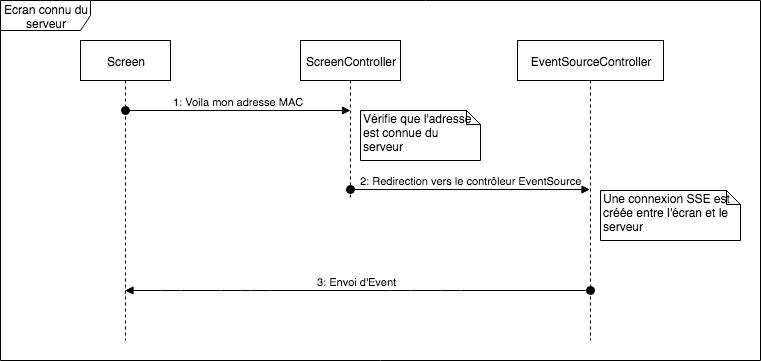
\includegraphics[scale=0.5]{schemas/screen_protocol.png}
		\caption{Protocole - écran connu par le serveur}
	\end{figure}

L'accès des écrans au serveur se fait donc en deux étapes. Il faut d'abord que l'écran se connecte à la route d'authentification des écrans, tout en spécifiant 
comme paramètre de requête son adresse MAC. Exemple:
\begin{verbatim}
	http://server/screens/auth?mac=1234
\end{verbatim}

Là, si l'adresse fournie est connue par le serveur, l'écran est redirigé vers le contrôleur chargé d'envoyer les Events aux écrans. Ce faisant, le ScreenController ajoute dans les cookies l'adresse MAC de l'écran ainsi que sa résolution (utile pour la gestion de l'affichage) et passe l'écran comme actif.

Ce protocole prend aussi en charge le cas où l'écran n'est pas connu du serveur. A ce moment là, il nous renvoie un code permettant l'ajout de l'écran dans le système depuis le site web. 

	\begin{figure}[h]
		\centering	
		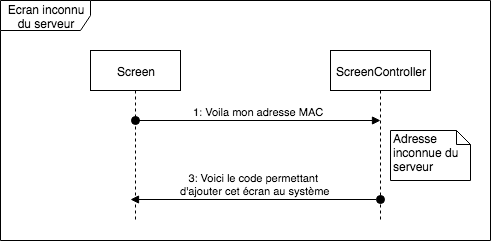
\includegraphics[scale=0.5]{schemas/screen_protocol_unknown.png}
		\caption{Protocole - écran inconnu par le serveur}
	\end{figure}
	
	Ce code est généré aléatoirement et unique pour chaque nouvel écran. Si l'écran essaie à nouveau de s'authentifier sans avoir été ajouté au système, le même code lui sera renvoyé. En cas de perte de connexion pendant l'échange, ce sera à l'écran de réitérer sa tentative. 
 
\subsubsection{Groupe d'écrans}
Une idée datant du début de ma réflexion sur le problème était de proposer à l'utilisateur de regrouper des écrans en groupes "logiques", par exemple le groupe des écrans du hall. Cela devait permettre d'assigner un Schedule à un groupe d'écrans et ainsi gagner du temps et rendre le programme plus simple. \newline
Malheureusement, c'est un détail qui m'a échappé lors de la réalisation de l'application. Quand j'ai remarqué mon oubli, il était trop tard pour l'intégrer car il aurait fallu changer plusieurs modèles ainsi que la base de données et le temps manquait.

\newpage
\section{Schéma de base de donnée}
Une des directives principales du projet était la représentation en tout temps de l'état actuel du programme en base de données. Le schéma a donc été pensé pour répondre à cette demande et les limitations voulues pour les différentes entités ont été au maximum intégrées dans la construction de la base. Dans les sections suivantes seront expliqués les choix et divers changements opérés pendant la phase d'analyse ainsi que des explications pour les éléments importants. Le schéma de la page suivante offre une représentation des tables et relations de la base de données et servira de référence dans ce chapitre.

\subsection{Equipes et utilisateurs}

Regrouper les gens en équipes permet de limiter le contenu auquel ils ont accès. La table Team est donc en relation avec toutes les entités manipulables, c'est-à-dire les écrans, Flux, Schedules et Diffusers pour filtrer les données envoyées à l'utilisateur. Comme mentionné dans le chapitre \textbf{Analyse et Architecture}, les équipes sont composées de membres simples et de chefs d'équipe (leur nombre n'est pas limité). Cette distinction permet de limiter les actions qui sont proposées par l'application selon le rôle de l'utilisateur (p.ex. restreindre la création de nouveaux Schedules aux chefs d'équipe mais laisser leur utilisation possible pour un membre). \newline
En ce qui concerne les utilisateurs, pour chacun d'entre eux existe une entrée de la table User qui contient leurs données personnelles (mot de passe, email). Cette table est "héritée" par TeamMember, qui contient une clé étrangère vers la table Team, et par Admin, qui représente un administrateur système. 

\subsection{Flux}

Dans les premières directives du projet figurait le besoin d'avoir des flux localisés et des flux généraux. Plus tard, toujours pendant la phase d'analyse, il a été jugé nécessaire de rajouter un modèle représentant les flux à envoyer lorsque le système détecte un problème avec le flux courant (envoi d'un flux localisé au mauvais site p.ex.). Comme pour les utilisateurs, il a été décidé de modéliser une relation "d'héritage" pour répondre à tout cela. Il y a donc une table Flux qui contient chaque flux créé (ses paramètres, type, etc). Les éléments de cette table ne peuvent pas être utilisé tels quels, il faut obligatoirement passer par les tables qui en héritent: 

\begin{itemize}
	\item \textbf{LocatedFlux}, qui représente un flux localisé et donc fait un lien entre Site et Flux.
	\item \textbf{GeneralFlux}, qui représente un flux général.
	\item \textbf{FallbackFlux}, pour les flux de fallback
\end{itemize}

\subsection{Schedule}

Pendant la réalisation du projet, j'ai du trouver une solution pour stocker en base de données les Schedules créés et surtout l'horaire choisi par l'utilisateur pour ses différents flux. Comme expliqué dans le chapitre \textbf{Analyse et Architecture} (section Schedule), j'ai d'abord mis au point une représentation d'une plage de diffusion en blocs d'une minute. Cette représentation n'étant pas satisfaisante, j'ai dû changer de méthode et ai donc ajouté trois entités de base de données : 
\begin{itemize}
	\item \textbf{FluxTrigger}: Signifie qu'un flux doit être envoyé à une certaine heure et sert de borne pour le Schedule.
	\item \textbf{FluxLoop} : Signifie qu'à partir d'une certaine heure, et jusqu'à la prochaine borne, les flux contenus dans la \textit{loop} seront bouclés indéfiniment. 
	\item \textbf{LoopedFlux} : Représente un flux faisant partie d'un \textit{FluxLoop}. Contient également une colonne supplémentaire servant à représenter l'ordre des flux dans la \textit{loop}.\newline
\end{itemize}   
Un Schedule doit également référencer ses flux de fallback afin d'être complet.\newline

Un Schedule doit pouvoir être activé et cette information doit être visible en base de données. Comme précisé dans le chapitre précédent, cette activation est représentée par la création d'une entité temporaire RunningSchedule, qui existe tant que le Schedule reste activé. Un Schedule ne possédant aucune référence vers des écrans, c'est le RunningSchedule qui contient ces informations. Outre cela, il ne contient qu'une référence vers son Schedule associé. \newline

Les Schedules contiennent également une String représentant les jours pour lesquels ils sont actifs (séparés par une virgule). 
    
\begin{landscape}
\begin{figure}[!h]
\centering
\fbox{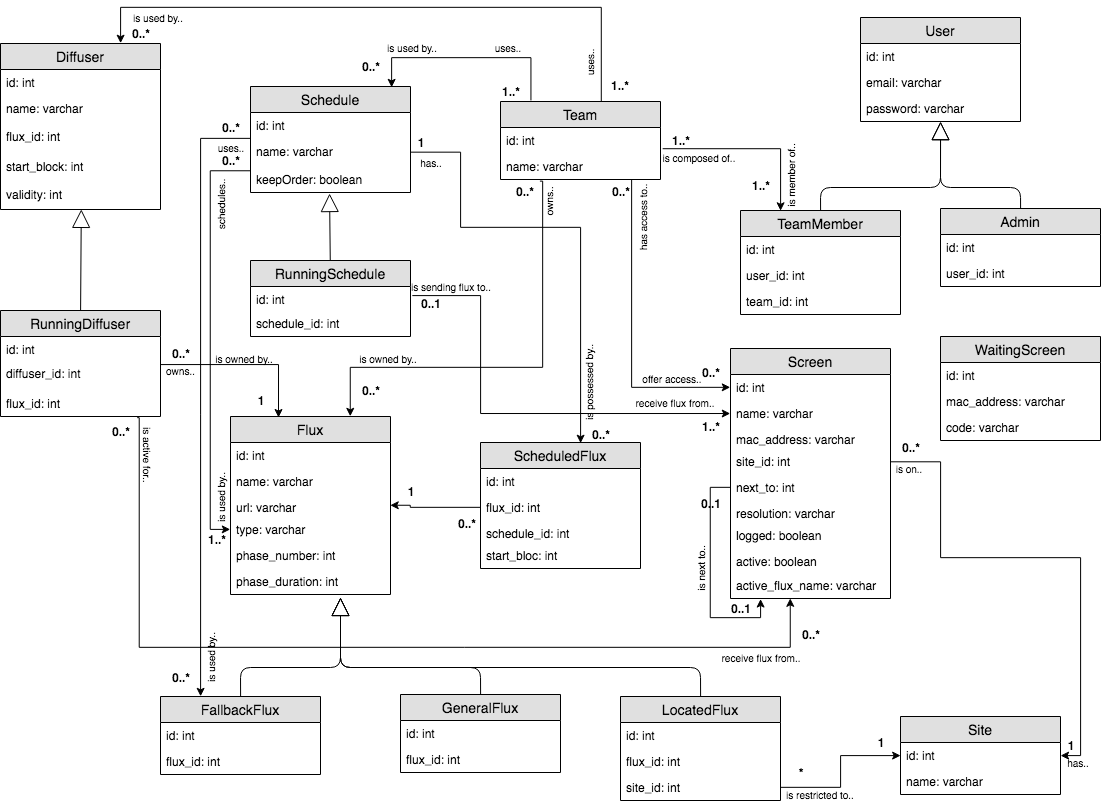
\includegraphics[scale=0.6]{schemas/db_schema_full}}
\caption{Schéma de la base de donnée}
\end{figure}
\end{landscape}
    
\newpage
\subsection{Diffuser}	

En termes de base de données, les Diffusers sont très similaires aux Schedules. Comme on doit également pouvoir activer un Diffuser, la même technique est utilisée, avec un RunningDiffuser créé à l'activation qui contient une référence vers les écrans concernés ainsi que le flux diffusé. Ils ont par contre quelques attributs en plus qui détermine leur comportement:
\begin{itemize}
	\item \textbf{Time}, qui contient l'heure de départ du Diffuser.
	\item \textbf{Days}, une String contenant les jours pour lesquels le Diffuser est actif (séparés par une virgule). \newline
\end{itemize}

Contrairement aux Schedules, les Diffusers contiennent directement ces informations car ils n'utilisent pas de \textit{FluxTrigger} ou de \textit{FluxLoop}.

\subsection{Ecrans}
Pour les écrans, la base de données est assez simple. Chaque entrée de la table représente un écran physique et donc contient des informations sur son lieu, son matériel et son état.  \newline
Une des demandes explicitées pendant les discussions avec mon mentor était d'avoir la possibilité de spécifier un voisin pour nos écrans (certains écrans de la HEIG-VD étant côte-à-côte). Ceci afin de ne pas afficher deux fois le même flux mais deux différents. Si cette information est modélisée en base de données, elle n'est pas utilisée dans le cadre de l'application.\newline
Il existe également la table WaitingScreen, qui représente un écran en attente d'enregistrement. Comme précisé dans le chapitre précédent, les nouveaux écrans inconnus du système qui essaient de d'authentifier reçoivent un code à fournir lors de leur ajout au système (en passant par l'interface). Entre le moment où le code est fourni et celui ou l'écran a été ajouté, une entrée de cette table fait le lien entre l'adresse MAC du nouvel écran et le code fourni par le serveur.

\newpage
\section{Architecture Logicielle}

\subsection{Architecture de Quartz}

En quelques mots, le concept primaire de Quartz est d'avoir un \textit{Scheduler} qui contient une liste de \textit{Jobs} qui sont activé à un certain moment par un \textit{Trigger}. Il est également possible d'enregistrer des \textit{Listeners} pour les \textit{Jobs} ou les \textit{Triggers} qui permettent d'effectuer des opérations avant ou après l'exécution d'un \textit{Job}. On peut voir les relations entre les différentes entités dans le schéma ci-dessous :

\begin{figure}[h]
	\centering	
	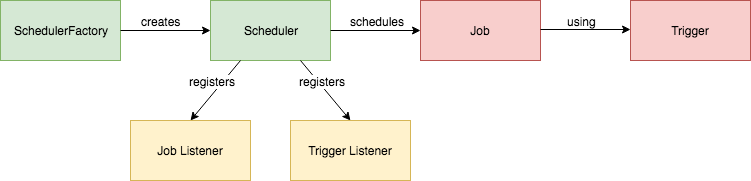
\includegraphics[width=0.8\linewidth]{schemas/quartz_arch.png}%
	\caption{Architecture de Quartz}
\end{figure}

\subsection{Utilisation de Quartz et Gestion des événements}
Dans le cadre du programme, l'envoi d'un événement à un écran est représenté par un \textit{Job}, qui s'occupera de traiter des données, un \textit{Trigger} qui s'occupera d'activer le \textit{Job} et qui contient diverses informations nécessaires à son exécution (les IDs des écrans concernés ou encore l'ID du flux à envoyer, etc) ainsi qu'un \textit{Listener} qui transmettra l'événement à l'EventManager. \newline

On peut observer dans le schéma de la page suivante l'architecture logicielle des différentes classes servant au traitement d'événements. Ce schéma sert de référence pour cette section.\newline

On peut observer ici plusieurs choses mais commençons par les \textit{Jobs}. Ils héritent de l'interface \textit{EventJob}, qui elle-même hérite de l'interface \textit{Job} de Quartz. Cette interface sert à forcer les \textit{Jobs} à implémenter quelques fonctions. Les deux types présents, soit \textit{SendEventJob} et \textit{SendLoopEventJob}, représentent respectivement un événement associé à un FluxTrigger et à un FluxLoop. Il est donc possible d'imaginer créer de nouveaux \textit{Jobs} associés à de nouvelles fonctionnalités. \newline
Concrètement, un \textit{Job} va récupérer les valeurs contenues dans le \textit{Trigger} l'ayant déclenché pour construire un FluxEvent représentant l'événement devant être envoyé aux écrans (un FluxEvent est composé d'un flux et de la liste des adresses MAC des écrans concernés par cet événement.). Il va également regarder quelle entité l'a déclenché (Schedule ou Diffuser). \newline

Maintenant que l'événement à été créé, il faut le transmettre aux écrans et c'est là que les \textit{Listeners} rentrent en action. De la même manière que pour les \textit{Jobs}, ils héritent de l'interface \textit{EventJobListener}, qui elle-même hérite de l'interface \textit{JobListener} de Quartz. A nouveau, cette interface sert à forcer les \textit{Listeners} à implémenter une fonction nécessaire. J'ai fait le choix d'avoir un type de \textit{Listener} par type de \textit{Job} car leur comportement n'est pas tout à fait le même selon le type d'événement traité. \newline
Cependant, tous les \textit{Listeners} effectuent les actions suivantes une fois qu'un \textit{Job} aie été exécuté:
ses informations sont récupérées, une vérification est effectuée pour savoir si le flux a du contenu à afficher et la suite du traitement est déléguée à l'EventManager. Leur comportement diffère quant au reste de leur exécution. Par exemple, un \textit{SendEventJobListener} va vérifier, après avoir envoyé l'événement à l'EventManager, quelle est la prochaine entrée du Schedule et si un FluxLoop est prévu, il va créer le \textit{Job} associé. Ces différences de fonctionnement seront explicitées dans le chapitre \textbf{Réalisation}. \newline

Le reste du traitement est effectué par l'EventManager (un singleton) qui reçoit tout les événements générés par le programme et les traite de manière accordée (détection de Diffuser actif, remplacement du flux prévu par un flux de fallback, etc). L'événement final est ensuite envoyé aux écrans par le biais de l'EventSourceController.

\newpage
\begin{figure}[h]
	\centering	
	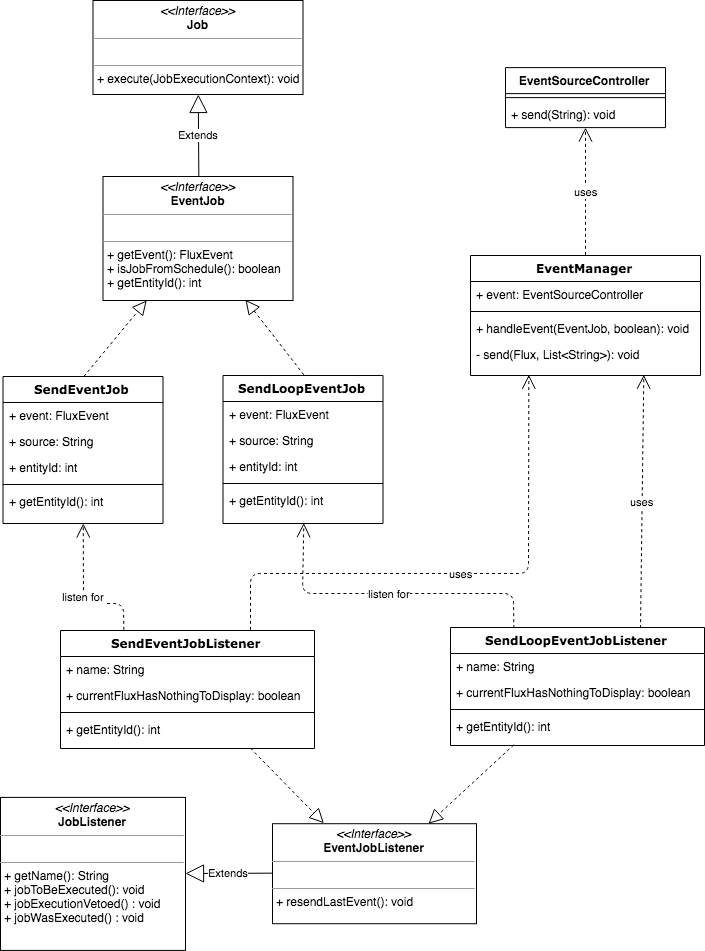
\includegraphics[width=0.9\linewidth]{schemas/event_handling.png}%
	\caption{Gestion des événements}
\end{figure}

Il convient de se demander pourquoi les \textit{Listeners} sont-ils utilisés et pourquoi les \textit{Jobs} ne pourraient-ils pas directement envoyer leur résultat à l'EventManager. Le problème vient de la structure de Play, en particulier l'obtention d'instances de classe par injection de dépendance. En effet, il est impossible pour les \textit{Job} d'utiliser l'injection de dépendance et il est également impossible de leur fournir des objets à leur création. Afin de palier à ce problème, j'ai donc utilisé les \textit{Listeners}. Je pense que c'est quand même une bonne chose car cela permet de plus facilement apporter des modifications ou nouvelles fonctionnalités.

\newpage
\subsection{Création de job}
En avançant dans la réalisation du programme, j'ai eu besoin de pouvoir créer ces \textit{Jobs} depuis différents endroit dans le code et avec des paramètres également différents selon l'entité les produisant (Schedule ou Diffuser). Pour répondre à ce besoin, j'ai mis au point des classes \textit{JobCreator}. On peut voir dans les deux schémas suivants les liens entre les différentes classes devant générer des \textit{Jobs} : \newline

\begin{figure}[h]
	\centering	
	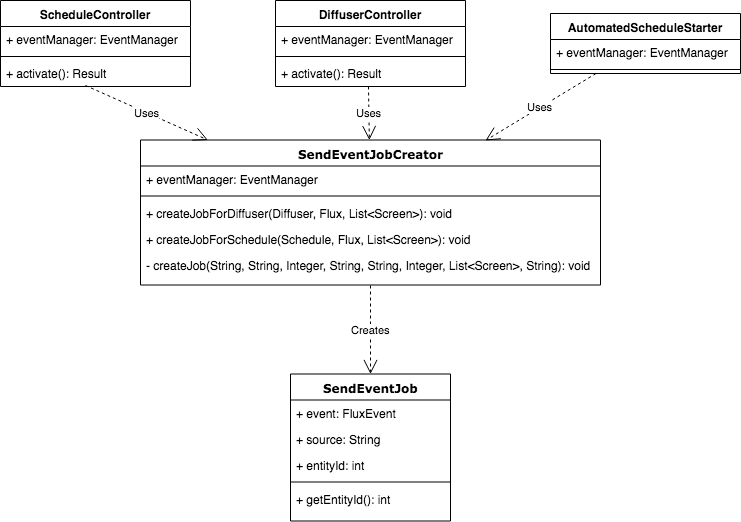
\includegraphics[width=0.7\linewidth]{schemas/job_creation.png}%
	\caption{Création de \textit{SendEventJob}}
\end{figure}

Les \textit{SendEventJob} peuvent être créés soit par un Schedule, soit par un Diffuser. La classe \textit{SendEventJobCreator} offre donc deux méthodes publiques, une pour les Schedules et une pour les Diffusers. un \textit{Job} est ensuite créé avec les bon paramètres.


\begin{figure}[h]
	\centering	
	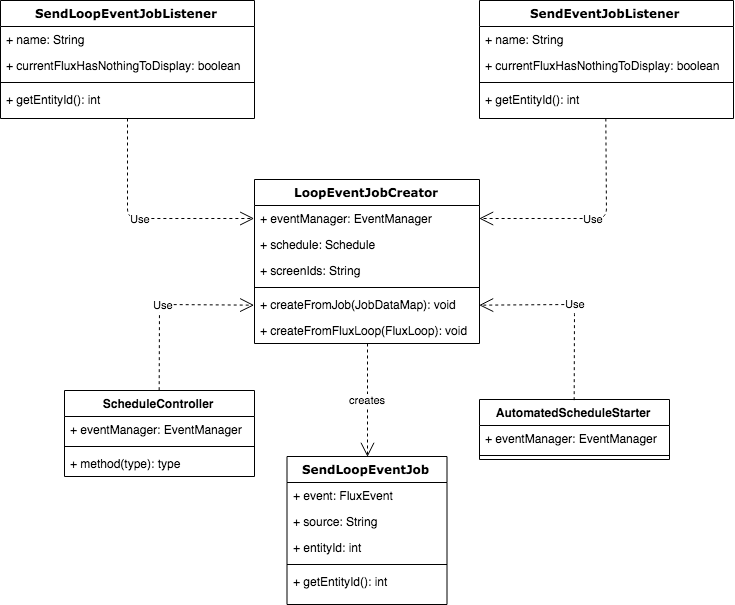
\includegraphics[width=0.7\linewidth]{schemas/loop_job_creation.png}%
	\caption{Création de \textit{SendLoopEventJob}}
\end{figure}

Le comportement du \textit{LoopEventJobCreator} est un peu différent du précédent car il ne peut être utilisé que dans le cadre d'un Schedule. Il offre deux méthodes publiques, \textit{createFromFluxLoop()} pour initier une nouvelle boucle et \textit{createFromJob()} pour continuer une boucle existante. \newline

\newpage
\subsection{DAO}
Voici un schéma simple décrivant l'architecture utilisée pour mes classes d'accès aux données :

\begin{figure}[h]
	\centering	
	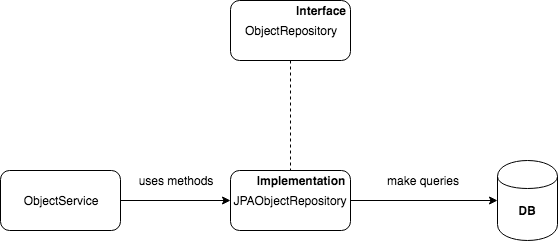
\includegraphics[width=0.8\linewidth]{schemas/dao_schema.png}%
	\caption{Schéma des services d'accès aux données}
\end{figure}

Dans cette figure, l'objet \textit{ObjectService} représente le service utilisé pour effectuer des opérations de base de données. Utiliser cette structure pour les DAO est recommandée par Play car elle regroupe la logique des fonctions d'accès aux données au même endroit et elle facilite grandement la mise en place de tests à base de mocks. 

\subsection{FluxChecker}

Voici un schéma décrivant mon idée d'implémentation pour vérifier si un flux a du contenu à afficher :

\begin{figure}[h]
	\centering	
	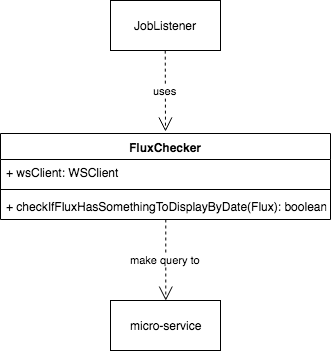
\includegraphics[width=0.5\linewidth]{schemas/fluxchecker.png}%
	\caption{Utilisation du FluxChecker}
\end{figure}

Dans l'exemple ci-dessus, le FluxChecker ne possède qu'une fonction, mais il est tout à fait envisageable d'en proposer plusieurs (une par type de validation). Il serait utilisé par les \textit{Listeners} pour vérifier le flux courant juste avant de l'envoyer à l'EventManager.

\newpage	
\section{Réalisation}

\subsection{Organisation des flux}


\subsubsection{Jobs et Listeners}

Comme expliqué dans le chapitre précédent, les \textit{Jobs} servent à construire l'objet FluxEvent qui sera utilisé par les \textit{Listeners} et l'EventManager. Dans l'extrait de code suivant, on peut observer la fonction \textit{execute()} de la classe \textit{SendEventJob} : 

\lstinputlisting[caption=SendEventJob.java, language=Java]{code/sendeventjob.java}

On voit que les trois attributs de la classe sont récupérés du \textit{Trigger} ayant déclenché le \textit{Job}. La \textit{source} sert à savoir quelle entité (Schedule ou Diffuser) a créer ce \textit{Job} et l'\textit{entityId} contient l'ID de cette entité.\newline

Une fois le \textit{Job} effectué, le \textit{Listener} approprié est activé et peut récupérer les valeurs construites dans le \textit{Job}. On peut voir dans l'extrait suivant la fonction \textit{jobWasExecuted()} de la classe \textit{SendEventJobListener} : 

\lstinputlisting[caption=SendEventJobListener.java, language=Java]{code/sendeventjob_listener.java}

Le premier point à noter est la fonction de vérification de flux qui demandera à un service externe si le flux courant a du contenu à afficher. Dans le cas contraire, on transmet quand même l'événement à l'EventManager mais avec un boolean false. Il se chargera ensuite de remplacer le flux par un flux de fallback. \newline
Jusque là, les deux \textit{Listeners} ont le même comportement, mais celui-ci diffère pour la suite. Dans l'exemple fourni, après avoir traité l'événement, le \textit{Listener} vérifie un FluxLoop est prévu après l'exécution du flux courant (ligne 30). Si oui, un \textit{SendLoopEventJob} est créé. Si non, et si le \textit{Job} venant d'être exécuté représentait le dernier FluxTrigger de la journée, le premier FluxLoop du Schedule est démarré. Si aucun FluxLoop n'existe pour le Schedule, rien ne se passe.

\subsubsection{Création de Jobs}

Comme expliqué précédemment, les \textit{Jobs} sont créés à l'aide d'une classe \textit{JobCreator} associée. On peut voir dans l'extrait suivant une partie du code de la classe SendEventJobCreator :

\lstinputlisting[caption=SendEventJobCreator, language=Java]{code/sendeventjob_creator.java}

On peut observer dans la troisième fonction (ligne 29), la manière dont les \textit{Jobs} et \textit{Triggers} de Quartz sont utilisés. Un SendEventJob est créé avec une identité et surtout un groupe d'appartenance (utile pour les \textit{Listeners}). Il est ensuite associé à un CronTrigger avant d'être "schedulé". Les différentes valeurs nécessaires aux \textit{Jobs} sont insérées dans une DataMap stockée dans le CronTrigger. \newline
On peut aussi observer la manière dont les \textit{Listeners} fonctionnent. J'ai fait le choix d'en avoir un par type de \textit{Job}. Ils sont donc identifiés par leur nom. \newline
A la ligne 68, on peut observer l'ajout d'un \textit{Listener} par le Scheduler de Quartz. C'est également à ce moment que l'on choisit quels seront les \textit{Jobs} écoutés par le \textit{Listener} nouvellement créé. Pour ce faire, il suffit de préciser un groupe de \textit{Jobs} (ligne 69). \newline
Pour le cas de la classe LoopEventJobCreator, le comportement est en partie identique, avec comme différences :
\begin{itemize}
	\item Les points d'entrée de la classe, qui cette fois ne dépendent pas de l'entité créant le \textit{Job} car seuls des Schedules peuvent posséder des FluxLoop. Il y en a un qui permet de commencer une boucle (\textit{createFromFluxLoop()}) et l'autre permettant de la continuer (\textit{createFromJob()}).
	\item La manière dont les valeurs nécessaires à la création des \textit{Jobs} et \textit{Triggers} sont obtenues (récupérées depuis le \textit{Job} précédent par exemple). 
\end{itemize}  

\subsubsection{EventManager}

L'EventManager est l'entité responsable de regrouper tout les événements générés par les Schedules et Diffusers pour les transmettre au contrôleur chargé de les envoyer aux écrans. C'est un Singleton qui est créé par injection de dépendance au démarrage de l'application et dont les contrôleurs ou autres objets peuvent obtenir une référence, par injection de dépendance à nouveau. Il reçoit des Events des différents Listeners actifs et les traite ensuite. C'est lui qui vérifie si un Diffuser est actif pour les écrans concernés par un événement et qui envoie les flux appropriés.\newline

C'est donc dans cette classe que la logique de "scheduling" est présente et que le choix du flux à afficher est effectué par le système. Quand l'EventManager reçoit un nouvel événement, il en vérifie avant tout la source (Schedule ou Diffuser) afin de le traiter correctement. Présenté ci-dessous, sa fonction \textit{handleEvent()}, qui sert de point d'accès à la classe :tet

\lstinputlisting[caption=Gestion des événements - EventManager.java, language=Java]{code/handle_event.java}

Si l'origine de l'événement est un Schedule, on passe par la fonction de la ligne 14. Elle se charge de vérifier que si le flux est localisé, les écrans concernés par l'événement soient sur le même site. Pour tout ceux étant localisés sur un site différent, un flux de fallback leur est envoyé à la place. Dans le cas où aucun flux de fallback n'a été choisi pour le Schedule, rien ne se passe pour ces écrans (ils continueront à afficher le dernier flux reçu).

Si le job vient d'un Diffuser, on passe cette fois directement dans la fonction \textit{sendFluxEvent()} à la ligne 18. Elle sert de "pré-point de sortie" de la classe, où les écrans ayant un Diffuser actif se voient envoyer le flux diffusé et les autres le flux prévu. 

\lstinputlisting[caption=Détection d'un Diffuser actif lors de l'envoi de Flux - EventManager.java, language=Java]{code/diffuser_detection.java}

Au lieu de modifier les Schedules avec les Diffusers, l'application peut  détecter qu'un RunningDiffuser est actif pour un écran auquel il s'apprêtait à envoyer un flux (vérification faites à la ligne 6 par la méthode \textit{sendDiffusedFluxToConcernedScreens()}) et ainsi modifier son comportement pour envoyer le flux diffusé et non le flux prévu. On peut observer cette méthode dans la figure suivante.

\lstinputlisting[caption=Envoi du flux diffusé aux écrans concernés - EventManager.java, language=Java]{code/send_diffused_flux.java}

On peut observer à la ligne 28 l'envoi du flux diffusé aux écrans concernés. Aux lignes 32 et 42, on construit petit à petit la String contenant les IDs des écrans non-concernés par un Diffuser. 

\newpage
\subsubsection{AutomatedScheduleStarter}

Grâce à Quartz, il devient très facile de reprendre l'exécution après un arrêt ou une maintenance du serveur car il suffit de re-générer les Jobs et Triggers de chaque Schedule actif et de les démarrer ensuite. Le code de cette classe est donc appelé au démarrage du programme (grâce aux annotations de Play) pour chaque RunningSchedule dans la base de données. La manière de faire étant la même que pour l'activation d'un Schedule, il n'y a pas d'exemple fourni.

\subsubsection{FluxChecker}

Le code présenté dans cette section n'a pas été testé car le service ou micro-serveur n'existe pas. Il s'agit uniquement d'une ébauche visant à mieux expliquer mon idée pour cette fonctionnalité.

\lstinputlisting[caption=FluxChecker, language=Java]{code/fluxchecker.java}

Cette classe sera utilisée par les \textit{Listeners} avant de transmettre l'événement à l'EventManager. Il avait été discuté avec mon mentor de vérifier les flux en amont, par exemple en vérifiant le prochain flux à chaque envoi de flux. Cependant, après réflexion, je suis venu à la conclusion que le programme et le micro-service s'exécuteront sur le même serveur. Le temps de réponse sera donc extrêmement bas (en dessous de la seconde) et le décalage sera donc minime et non perceptible. Il faudra bien sûr s'assurer de plusieurs choses pour faire cette hypothèse :
\begin{itemize}
	\item Le micro-service devra être rapide et sans-faute. Idéalement, il devrait garder à jour plusieurs listes de flux n'ayant potentiellement rien à afficher, une par type de vérification (voir chapitre \textbf{Analyse et Architecture}, section 4.3.1).
	\item La vérification depuis le programme devra être non-bloquante. Si le micro-service ne répond pas ou si un problème de connexion survient, l'envoi du flux devrait se poursuivre et l'exécution du programme ne devrait pas être interrompue.
\end{itemize}
 
\newpage
\subsection{Contrôleurs}

La plupart des contrôleurs de l'application servent uniquement à exécuter des opérations CRUD, mais certains offrent des fonctionnalités plus poussées qui sont décrites dans les sections suivantes. 

\subsubsection{EventSourceController}

Lors des discussions préalables avec mon mentor, j'avais été prévenu que dans la version 2.7 de Play Java, les Eventources ne fonctionnaient pas car les informations de session étaient perdues lors d'un mapping. Travaillant avec la version 2.7.1 (sensée avoir résolu ce problème), je suis donc parti sur une implémentation en Java. J'ai d'abord pensé avoir réussi, car j'observais un comportement normal, mais en analysant de manière plus approfondie les échanges clients-serveurs lors d'une séance avec mon mentor, nous nous sommes aperçu que la connexion Eventsource était recréée toutes les 3 secondes, quand le client essayait de se reconnecter au serveur. Il a donc été nécessaire de passer à une version en Scala.\newline
Ci-dessous une version simplifiée de l'ancien code Java:

\lstinputlisting[caption=Eventsource Java - EventSourceController.java, language=Java]{code/eventsource.java}

L'idée de ce contrôleur était de mettre à jour une source à chaque fois qu'un événement était envoyé grâce au patron de conception \textit{Observer}. 
\newpage

Après un peu de recherche sur les différents moyen d'implémenter une utilisation des Eventsource en Scala, j'ai choisi une solution basée sur les Akka Actor. Elle semblait la plus simple et la plus adaptée à mon problème, car elle permet de représenter chaque écran par un acteur. \newline
Le contrôleur équivalent en Scala:

\lstinputlisting[caption=Eventsource Scala - EventSourceController.scala, language=Scala]{code/eventsource.scala}

On peut voir que ce contrôleur est au final très simple. Il offre deux actions principales: la possibilité pour un écran de s'enregistrer auprès du manager grâce à la méthode \textit{events()} et un moyen pour le système d'envoyer un événement aux écrans avec la méthode \textit{send(event: String)}. \newline
Il utilise pour ce faire un ActorSystem, construit à l'aide d'une sous-classe d'Actor, créée dans le cadre du projet. En voici l'implémentation:

\lstinputlisting[caption=Akka Actor Scala - EventSourceController.scala, language=Scala]{code/actors.scala}

\subsubsection{ScreenController}

\paragraph{Authentification}

C'est par ce contrôleur que passe les écrans souhaitant s'authentifier auprès du système et ainsi recevoir des flux. La logique du comportement étant décrite dans le chapitre \textbf{Analyse et Architecture}, seul l'implémentation sera évoquée ici. \newline
Voici la version simplifiée de cette fonction:
\lstinputlisting[caption=Authentification des écrans - ScreenController.java, language=Java]{code/authenticate.java}

On s'aperçoit que son fonctionnement est assez simple: si l'écran n'a pas encore été ajouté au système, une entité WaitingScreen est créée (ou existe déjà) avec la même adresse MAC et le code est envoyé à l'écran. Sinon, l'écran est simplement redirigé vers l'EventSourceController après lui avoir rajouté des cookies. Dans le cas où le serveur ne détecte aucun Schedule actif pour cet écran, il est redirigé vers une page d'erreur.

\paragraph{Désactivation}

Il pourrait arriver de vouloir arrêter l'affichage sur un écran en particulier sans pour autant stopper le Schedule associé et continuer l'affichage sur les autres écrans. J'ai donc du mettre au point une manière d'enlever un écran de la liste des écrans concernés par un Schedule. La fonction permettant ceci est disponible dans une version simplifiée ci-dessous: 

\newpage
\lstinputlisting[caption=Désactivation des écrans - ScreenController.java, language=Java]{code/screen_deactivation.java}

Elle revient à simplement enlever l'écran visé de la liste des écrans concernés par le Schedule. Cette fonctionnalité manque de tests et il est donc possible d'avoir des comportements curieux. Actuellement, elle ne fonctionne que pour les FluxLoop.

\subsubsection{ScheduleController}

Ce contrôleur, en plus d'offrir des opérations CRUD sur les Schedules, permet de les activer et désactiver. Ce sont ces deux fonctionnalités qui seront décrites dans les sections suivantes. Le code présenté est à nouveau simplifié; les diverses vérifications faites sur les données ou sur l'état du programme ne sont par exemple pas présentes.

\paragraph{Activation}

L'activation d'un Schedule se fait en deux étapes principales. On crée d'abord un objet RunningSchedule à partir du Schedule à activer. On itère aussi à travers les écrans concernés par ce Schedule afin mettre à jour quelques valeurs. Dans la deuxième partie (ligne 25), les \textit{Jobs} et \textit{Triggers} de Quartz sont créés et lancés.

\lstinputlisting[caption=Activation d'un Schedule - ScheduleController.java, language=Java]{code/schedule_activation.java}

La fonction \textit{createJobsForSchedule()} récupère de la base de données les FluxTriggers du Schedule à activer et pour chacun d'entre eux schedule un \textit{SendEventJob}. Elle vérifie aussi si la première entrée du Schedule est un FluxLoop et, le cas échéant, schedule également un \textit{SendLoopEventJob}.


\paragraph{Désactivation}

La désactivation est quant à elle bien plus simple, car elle se résume à supprimer de la base de données le RunningSchedule visé et à supprimer les \textit{Jobs} et \textit{Triggers} de Quartz créés pour ce Schedule (effectué par la méthode \textit{deleteJobsOfSchedule()} à la ligne 11).

\lstinputlisting[caption=Désactivation d'un Schedule - ScheduleController.java, language=Java]{code/schedule_deactivation.java}

La fonction \textit{deleteJobsOfSchedule} parcourt à nouveau la base de données pour récupérer les FluxTriggers du Schedule et pour chacun d'eux, supprimer le \textit{Job} associé. Elle supprime également un potentiel \textit{SendLoopEvenJob}. 


\subsubsection{DiffuserController}

Ce contrôleur offre des opération CRUD sur les Diffusers et permet de les activer et désactiver. \newline
L'activation d'un Diffuser à été une des fonctionnalités les plus dures à implémenter. Je voulais en effet les connecter entièrement avec mes Schedules et les faire utiliser le même système d'horaire. Une fois celui-ci défini et testé avec les Schedules, j'ai commencé à réfléchir aux Diffusers. Je me suis aperçu qu'il fallait les différencier en deux types: standard et urgent. Pour le type standard, le flux diffusé est rajouté dans l'horaire du Schedule associé à l'écran si possible et pour l'urgent, le flux est diffusé immédiatement puis l'exécution reprend son cours habituel. \newline
C'est en tout cas ce que j'ai fait avant de réaliser que mon système ne fonctionnait pas. En effet, pendant la rédaction de ce rapport, j'ai remarqué qu'un Schedule peut être activé sur plusieurs écrans et donc modifier tout un Schedule pour un écran générera des effets de bords en modifiant l'affichage sur des écrans non-choisis. Mes deux types de Diffusers utilisant la même logique sous-jacente (à savoir modifier l'horaire d'un Schedule actif), ils sont donc tout les deux inutiles. Je suis passé à côté de ce détail pendant tout le semestre car pendant mes tests je travaillais avec des Schedule contenant peu d'écrans et ce cas de figure n'était jamais arrivé.\newline
Ma logique initiale était fausse; je n'aurais pas du essayer de mixer les Schedules et Diffusers, trop de problèmes sont survenus à cause de cela. Afin de palier un peu à ce problème, j'ai effectué des modifications de dernière minute afin d'avoir quand même un Diffuser fonctionnel, en tout cas une première implémentation. \newline
L'activation d'un Diffuser est désormais représentée par l'ajout dans la base de donnée d'un RunningDiffuser. A chaque fois qu'un événement est envoyé aux écrans, le système vérifie si un RunningDiffuser existe pour ces écrans. Si oui, il leur envoie le flux diffusé et si non, il continue l'exécution normale de son Schedule. Grâce à cela, une séparation est faite entre Diffuser et Schedule, le premier étant prioritaire sur l'autre. Dans le cas où l'écran choisit pour le Diffuser n'est pas assigné à un Schedule actif, un \textit{Job} est créé pour diffuser le flux à la bonne heure.


\paragraph{Activation/désactivation}

Dans l'extrait de code suivant figurent des versions simplifiées des fonctions d'activation et désactivation des Diffusers :

\newpage
\lstinputlisting[caption=Activation d'un Diffuser - DiffuserController.java, language=Java]{code/diffuser_activation.java}

On peut voir dans la partie \textit{activation}, aux lignes 24 à 35, la création d'un \textit{Job} pour les écrans n'ayant pas de Schedule actif. On peut aussi voir dans la deuxième partie que la désactivation d'un Diffuser revient à supprimer de la base de données le RunningDiffuser associé et supprimer les \textit{Jobs} du Scheduler de Quartz (ligne 51).

\newpage
\subsection{DAOs}

Dans cette section sera décrite l'implémentation des services d'accès à la base de données, ou \textbf{DAO} (pour DataAccessObject). 

\subsubsection{Requêtes SQL}

Les requêtes à la base de données sont effectuées dans le cadre d'une transaction, ce qui permet de roll-back en cas d'erreur et ainsi de ne pas modifier la base de données avec de fausses valeurs. J'utilise l'injection de dépendance afin d'obtenir un objet JPAApi, qui offre des moyens simples et efficaces d'écrire des requêtes SQL. On peut voir ci-dessous un exemple des méthodes standards d'insertion, mise-à-jour, récupération et de suppression:

\lstinputlisting[caption=Exemples de requêtes SQL avec JPA, language=HTML]{code/sql_requests.java}

On peut observer que la ressource JPA est obtenue par injection de dépendance et offre des raccourcis très pratiques avec son EntityManager, par exemple pour insérer des données avec la méthode \textit{persist()}. Il est bien sûr aussi possible d'écrire des requêtes natives comme pour la fonction \textit{get(String email, String password)}.

\subsubsection{Services}

Les services regroupent les fonctions d'accès aux données par type de données. Par exemple, un FluxService offre des méthodes d'ajout, de suppression mais aussi une fonction qui retourne la liste de tous les flux d'une Team précise. Ils contiennent aussi des fonctions de "casting", par exemple pour récupérer non pas une liste de Flux mais plutôt une liste de FluxData, utile pour l'affichage de vues.\newline
Dans le cadre de cette application, ils sont générés à la demande par un objet ServicePicker, qui utilise l'injection de dépendance pour créer les différents service selon le besoin. Ci-dessous un extrait de code montrant la manière dont les services sont fournis par la classe \textit{ServicePicker.java}

\lstinputlisting[caption=Exemple de création de service, language=HTML]{code/service_picker.java}

\subsubsection{Implémentation Java des entités BD}

Pour lier une classe Java et une table de base de données SQL, on utilise des annotations pour expliciter les relations entre attributs et colonnes. Dans l'extrait de code suivant, on peut voir une version simplifiée du modèle Schedule:

\lstinputlisting[caption=Exemple de modèle Java - Schedule.java, language=HTML]{code/schedule_dbmodel.java}

Plusieurs choses sont à noter:
\begin{itemize}
	\item Des annotations sont utilisées pour permettre à Play de faire correctement les liens avec les tables et colonnes de la base de données. Par exemple les \textit{@Table} et \textit{@Column}, où le nom est indiqué.
	\item Comme les IDs des objets en base de données sont du type SERIAL, la stratégie de la génération de l'identité doit être \textit{GenerationType.IDENTITY}.
	\item L'attribut \textit{fluxes} représente la liste des flux d'un Schedule et doit donc être annoté avec un \textit{@ElementCollection}. Cet attribut ne correspondant pas immédiatement avec une colonne de la table Schedule, il faut lui préciser sa stratégie de récupération de données comme \textit{EAGER}. En effet, le comportement standard est du type \textit{LAZY} et comme les données n'existent pas dans la table Schedule mais dans la table schedule\_fluxes, une évaluation paresseuse rendra des données nulles ou une erreur.
	\item Il faut fournir un constructeur sans paramètres.
\end{itemize}

Egalement à noter : pour certain objets représentant une table ne possédant pas d'ID propre mais d'un ID composite, une classe représentant cette composition doit être implémentée et l'ID de l'objet en question doit être du type de cette classe.

\subsection{Restriction d'accès}

Certaines vues ou fonctionnalités peuvent être limitées à une ou plusieurs catégories d'utilisateurs. Ces restrictions ont été implémentées en utilisant des Actions. Une Action est basiquement une fonction qui analyse les paramètres d'une requête et produit un résultat qui est renvoyé au client. Comme il s'agit d'une fonction, il est très facile de composer plusieurs actions ensemble. On peut dès lors construire une action qui va vérifier les paramètres de la requête pour récupérer un cookie d'authentification et selon la valeur de ce cookie, passer à l'Action suivante ou être redirigé ailleurs. Comme un exemple est bien plus parlant, voici l'Action vérifiant si l'utilisateur courant est un admin :

\lstinputlisting[caption=Admin Authentification Action, language=Java]{code/action_admin.java}

On peut voir que la méthode principale de cette classe, \textit{call()}, vérifie simplement si le cookie "email" existe, et dans l'affirmative, s'il correspond à l'email d'un admin. Si oui, il continue son exécution et passe la main (délègue) à l'Action suivante. Si non, il renvoie à la page de login avec un message d'erreur. Cette Action est ensuite utilisée de la manière suivante :

\newpage
\lstinputlisting[caption=Utilisation d'une Action custom, language=Java]{code/action_usage.java}

L'annotation \textbf{@With} permet de spécifier que l'on souhaite passer par une autre Action avant d'exécuter le contenu de la méthode \textit{index()}.

\subsection{Triggers}

Comme la majorité des tables intermédiaires (par exemple team\_fluxes) ont des références non nulles vers des lignes d'autres tables, la suppression de l'une de ces lignes entrainait des erreurs de transaction et l'annulation de l'opération en cours. J'ai donc du mettre en place des triggers SQL qui s'occupent d'effacer les lignes des tables intermédiaires lorsque nécessaire. Les entités concernées sont toutes celles possédant une clé étrangère non nulle. Ces triggers étant sensiblement tous les mêmes, un seul exemple est fourni:

\lstinputlisting[caption=Triggers SQL - Suppression, language=SQL]{code/triggers_delete.sql}

Le trigger est appelé avant l'opération de DELETE pour qu'il s'exécute avant que l'erreur n'apparaisse. 

J'en utilise également un autre qui se déclenche cette fois après une insertion dans la table TeamMember pour ajouter le nouveau membre dans la liste des membres de la Team correspondante.\newline

J'ai conscience que le projet étant plutôt axé sur la modélisation et la base de données, il aurait bénéfique d'avoir des triggers servant à la validation/vérification des données insérées afin d'être entièrement sûr de la cohérence de la base.

\newpage
\subsection{Vues}

Ce chapitre décrit la manière dont les différentes vues de l'application ont été construites. Elles font usage des fonctionnalités proposées par Play, par exemple des helpers qui facilitent la construction de divers objets Bootstrap ou l'injection de code Scala dans les fichiers HTML.

\subsubsection{Affichage des flux}

L'affichage des Events reçus par les écrans se fait à l'aide d'une page HTML simple, qui défini les balises nécessaires à l'affichage des différents types de flux. A part un peu de CSS, rien d'autre ne s'y passe. En voici le body:

\lstinputlisting[caption=Eventsource HTML, language=HTML]{code/eventsource.html}

Il est couplé d'un script Javascript qui créé la connexion SSE avec le serveur et qui traite les Events qu'il reçoit par la suite. Selon le type de flux, il appelle des fonctions d'affichage différentes, qui agissent avec JQuery sur les balises présentées précédemment pour en modifier le contenu ou les cacher. Ci-dessous est présenté la fonction principale de ce script:

\lstinputlisting[caption=Eventsource JS, language=java]{code/eventsource.js}

On peut observer dans la déclaration de la fonction de Listening de notre Eventsource la logique de déconstruction des messages reçus, ainsi que le traitement adéquat selon le type du flux.


\subsubsection{Echange de données}

Pour échanger des informations entre le serveur et le client, j'ai choisi  d'utiliser les fonctionnalités offertes par Play, donc avoir des entités représentant mes données (par exemple un Flux devient un FluxData) et de les utiliser avec les templates Scala, Play permettant de facilement transférer des objets Java des contrôleurs aux vues. Ces templates sont des blocs de texte contenant du code Scala qui est par la suite compilé en HTML. Il devient alors facile de combiner cela à Bootstrap pour l'affichage ou l'envoi de données depuis le client.

Exemple d'entité:
\lstinputlisting[caption=UserData.java, language=java]{code/userdata.java}


\paragraph{Serveur -> client}

\lstinputlisting[caption=Exemple échange serveur-client, language=java]{code/server_to_client.java}

Ici, \textit{datautils.getAllTeams()} renvoie une liste liste de \textbf{TeamData} qui sont récupérés et utilisés ensuite par le fichier HTML. On peut observer ici l'intégration d'une boucle for Scala avec une Table Bootstrap.

\newpage
\paragraph{Client -> serveur}

\lstinputlisting[caption=Exemple échange client-serveur, language=java]{code/client_to_server.java}

Dans cet extrait de code, on a un exemple des fonctionnalités offertes par Play sous la forme de helpers servant à faciliter la création de formulaires Bootstrap. L'action effectuée par le bouton du formulaire est directement liée à la méthode de UserController.java. Il faut choisir comme valeur pour l'attribut name des balises <input> les noms des attributs correspondants dans le modèle associé (UserData en l'occurence).\newline
Le serveur est par la suite capable de reconstruire un objet du même type en récupérant le formulaire depuis la requête.

\paragraph{Erreurs}

Parmi les exigences du projet figurait la nécessité d'empêcher l'utilisateur de faire des fausses manipulations sur les données et surtout de l'informer en cas d'erreur de l'application avec des messages utiles. Il a donc fallu trouver un système permettant d'afficher facilement un message dans les vues de l'application en cas d'erreur. \newline

Ci-dessous, un extrait de trois fichiers explicitant le traitement des erreurs dans l'application:

\lstinputlisting[caption=Exemple des messages d'erreur, language=java]{code/erreurs.java}

Les contrôleurs ont à chaque fois deux méthodes pour retourner une vue, une sans message d'erreur et une avec (lignes 2 à 9). Même si certaines de ces méthodes sont identiques, il peut être utile de séparer la logique d'affichage en cas d'erreur pour potentiellement effectuer des opérations supplémentaire ou envoyer des données différentes. \newline
Ce message d'erreur est récupéré par la vue correspondante, dans notre cas: \textit{user\_page.scala.html}, qui l'envoie ensuite au template main. Ce template est appelé avant chaque vue et définit entre autre des headers, styles, etc. Il contient également le troisième extrait de code du Listing précédent. Ce code affiche une alerte avec comme message l'erreur envoyée par le serveur. Cette implémentation permet de simplifier le traitement des erreurs en regroupant toute la logique frontend au même endroit et en offrant des méthodes simples d'utilisation pour le serveur.

\newpage
\section{Interface}

Dans cette section sera présentée et expliquée la version finale de l'interface utilisateur. \newline
La navigation dans les différentes pages de l'application est organisée avec une Navbar Bootstrap. Chacune des sections suivantes décrit une de ces pages.  

\subsection{Home}

Cette page sert de page d'accueil dans le programme et affiche les écrans, Schedules et Diffusers actifs dans des Tables Bootstrap. Elle permet également d'arrêter la diffusion en cours sur un écran en le désactivant à l'aide d'un bouton.

\begin{figure}[h]
	\centering	
	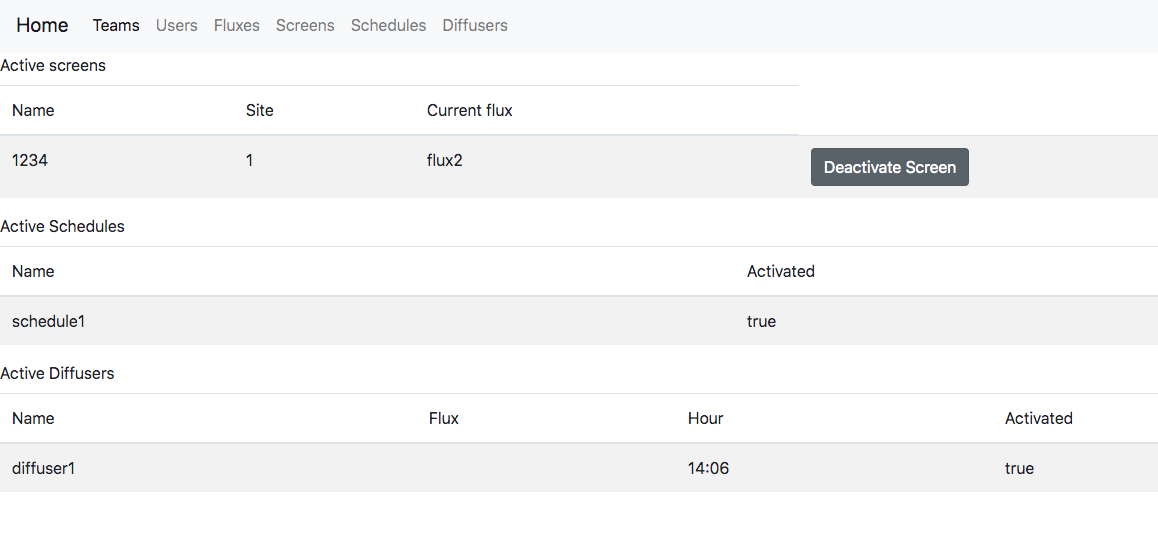
\includegraphics[width=0.8\linewidth]{interface/homepage.png}%
	\caption{Homepage}
\end{figure}

Cette technique d'affichage des données avec des Tables est celle utilisée pour toutes les pages principale de l'application, soit celles accessibles par la Navbar.

\subsection{Teams}

Cette page est uniquement accessible par un admin car depuis elle, on a accès à toutes les teams existantes, avec la possibilité de les mettre à jour ou des les supprimer. On peut également  créer une nouvelle team et cette page est un peu particulière car toutes les données y sont accessibles. Un admin peut en effet vouloir directement spécifier des Flux ou utilisateurs ou autre entité lors de la création, donc les données envoyées ne sont pas limitées par la Team de l'utilisateur courant (c'est logique, seul l'admin y a accès). 

\begin{figure}[h]
	\centering	
	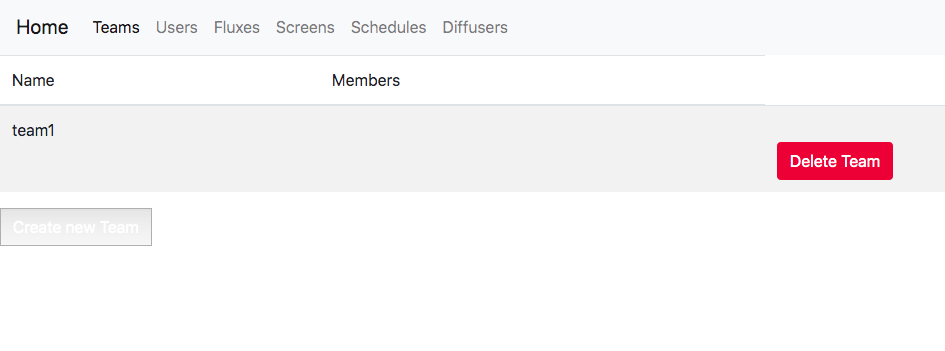
\includegraphics[width=0.8\linewidth]{interface/teampage.png}%
	\caption{Teampage}
\end{figure} 

\newpage
\subsection{Users}

Cette page est accessible par les admins et les chefs d'équipe. Elle référence les utilisateurs inscrits dans le système et permet leur mise à jour ou suppression. Elle offre aussi un lien vers la page d'ajout d'utilisateur, qui est présentée ci-dessous :

\begin{figure}[h]
	\centering	
	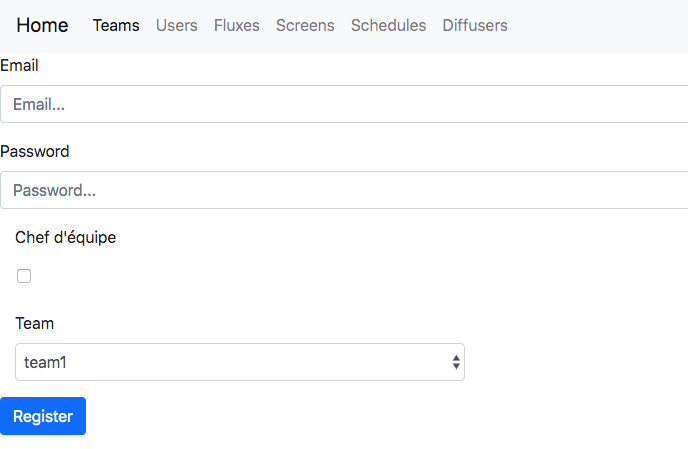
\includegraphics[width=0.8\linewidth]{interface/userpage_register.png}%
	\caption{Ajout d'utilisateur}
\end{figure} 

Il n'y a pas besoin d'être authentifié pour accéder à cette page car elle est utilisée pour se créer un compte. On peut préciser la team dont il fait partie et s'il s'agit d'un chef d'équipe.

\subsection{Fluxes}

De la même manière que les autres, cette page présente les flux accessibles par l'utilisateur courant et permet de les modifier, supprimer ou d'en créer des nouveaux. C'est l'interface de création qui sera présentée dans cette section :

\begin{figure}[h]
	\centering	
	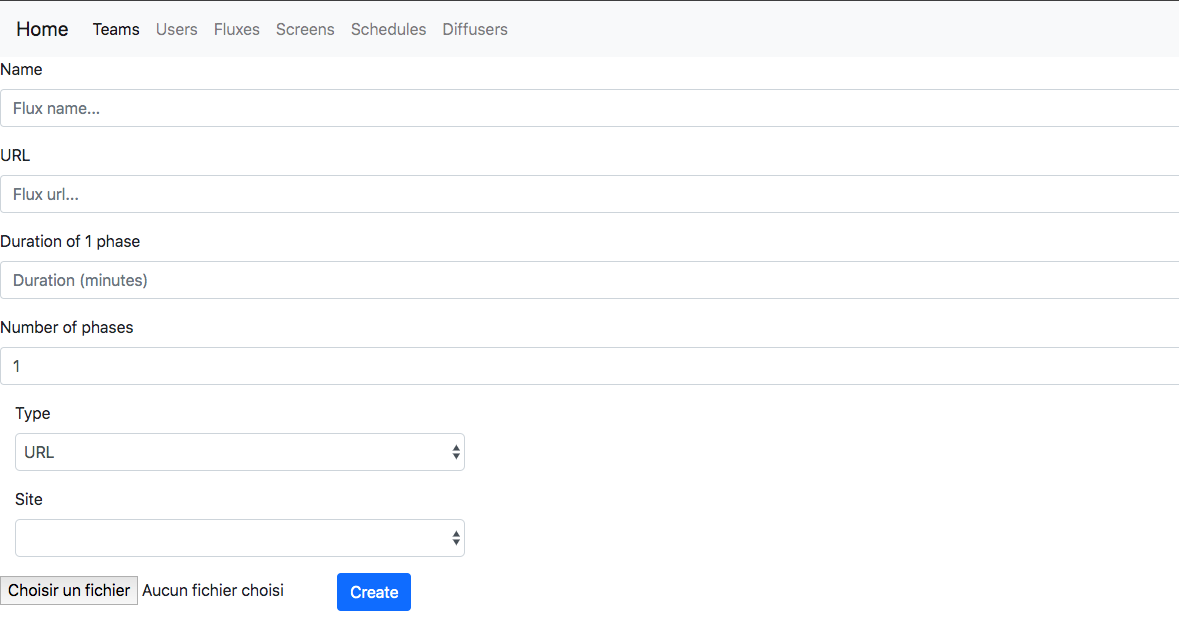
\includegraphics[width=0.8\linewidth]{interface/fluxpage_creation.png}%
	\caption{Création de Flux}
\end{figure} 

On y voit les différents moyens de création de flux. J'aurais voulu changer le formulaire affiché selon le type de flux créé (URL, VIDEO, etc), car pour l'instant, tous les champs sont accessibles tout le temps. Voici la procédure minimale à suivre par type :
\begin{itemize}
	\item \textbf{URL}: entrer l'URL de la page à afficher et choisir une durée.
	\item \textbf{IMAGE}: choisir une durée et uploader une image.
	\item \textbf{VIDEO}: entrer l'URL de la vidéo Youtube à afficher et choisir une durée.
	\item \textbf{TEXT}: entrer le texte à afficher dans le champs URL et choisir une durée 
\end{itemize}
Pour chacun de ces choix, il est également possible de choisir un Site et ainsi créer un flux localisé.

\subsection{Screens}

Cette page présente les différents écrans accessibles par la Team de l'utilisateur courant et offre les mêmes fonctionnalités que les autres pages : mise à jour, suppression, ajout d'écran au système. La seule particularité de cette section est d'exiger un code d'authentification pour l'ajout d'écran.

\subsection{Schedules}

Cette page est un peu spéciale car en plus des habituelles opérations CRUD proposées, elle offre aussi la possibilité d'activer et de désactiver les Schedules, comme on peut le voir sur la figure suivante :

\begin{figure}[h]
	\centering	
	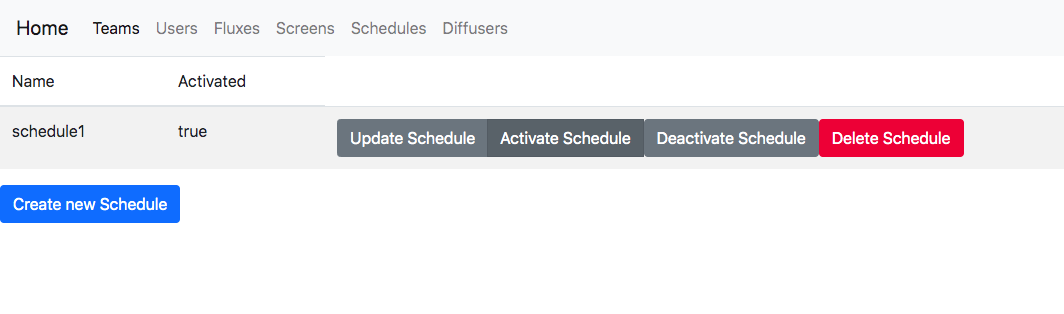
\includegraphics[width=0.8\linewidth]{interface/schedulepage.png}%
	\caption{Schedules page}
\end{figure} 

Ce bouton nous redirige vers une autre vue, qui elle permet de choisir les écrans qui seront concernés par ce Schedule. Les écrans affichés dans la liste sont les écrans accessibles par la Team de l'utilisateur courant.

\begin{figure}[h]
	\centering	
	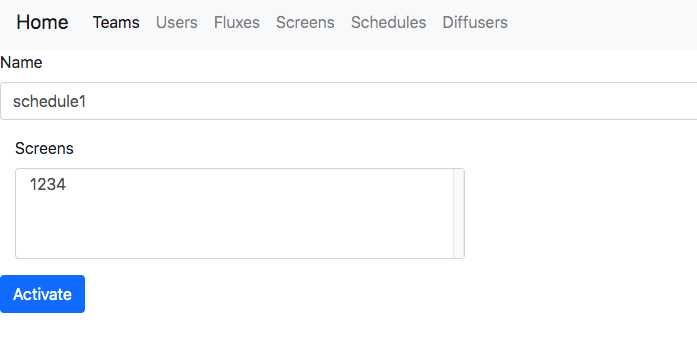
\includegraphics[width=0.8\linewidth]{interface/schedulepage_activation.png}%
	\caption{Schedules page}
\end{figure} 
\newpage
La page la plus compliquée que j'ai eu à réaliser fût celle permettant la création de Schedules. Il fallait en effet trouver un moyen de choisir les flux composant le Schedule et pour chacun de ces flux avoir la possibilité de définir une heure de début. Ayant assez peu d'expérience en \textit{frontend} de manière générale, j'ai beaucoup cherché d'idées en ligne et ai fini par trouver un exemple que j'ai pu adapter à mon problème. En associant une Table Bootstrap avec du Javascript, je suis arrivé au résultat présenté dans la figure suivante :

\begin{figure}[h]
	\centering	
	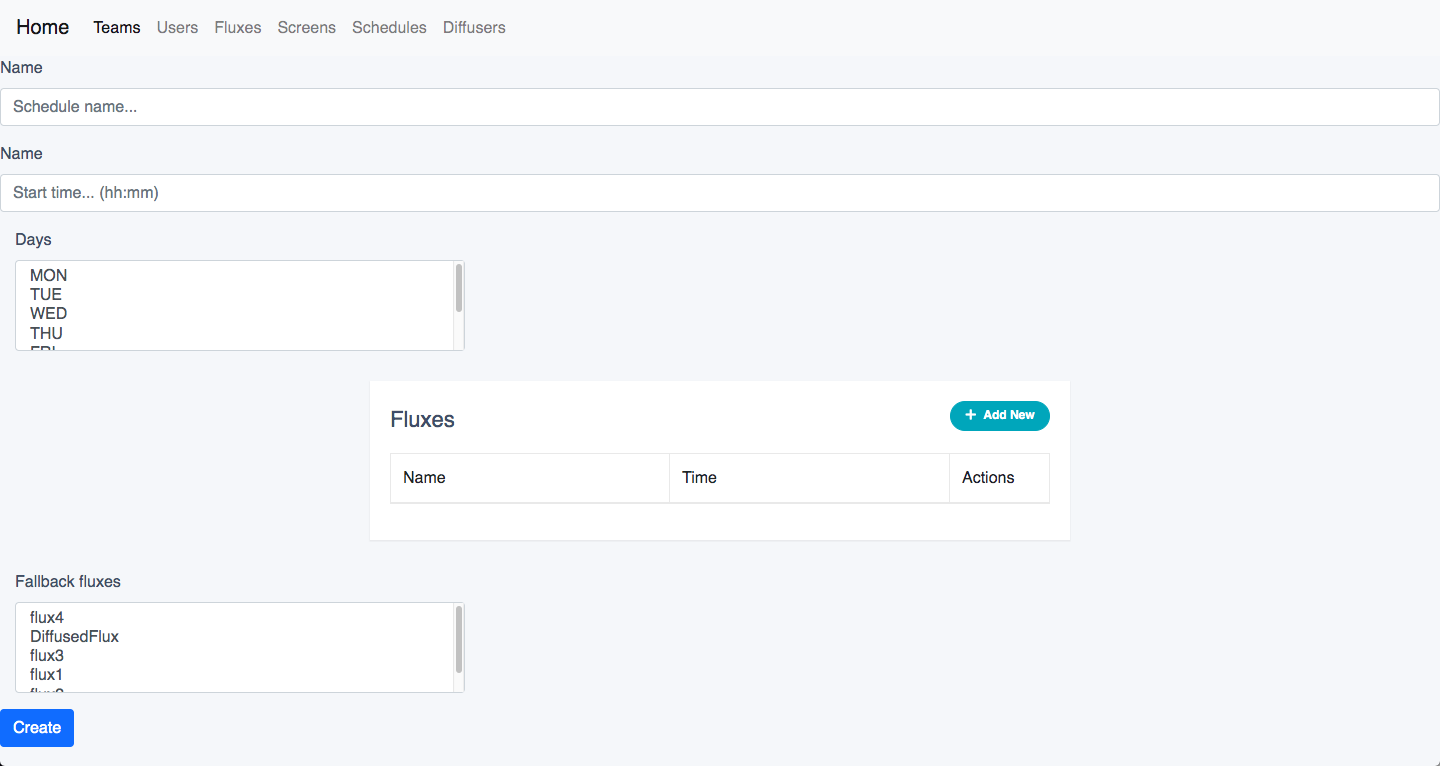
\includegraphics[width=0.8\linewidth]{interface/schedulepage_creation.png}%
	\caption{Schedules page}
\end{figure} 

On peut observer trois parties à cette page :
\begin{itemize}
	\item Une pour le choix des jours d'activité du Schedule (si aucune valeur n'est sélectionnée, cela veut dire qu'il sera actif tout les jours de la semaine).
	\item Une pour l'ajout de flux (avec heure de début ou non) au Schedule.
	\item Une pour le choix des flux de fallback du Schedule.
\end{itemize}
En cliquant sur le bouton \textit{Add new}, une nouvelle ligne apparait dans le tableau. Dans la colonne \textit{Name}, on peut choisir parmi les flux disponibles pour la Team courante et dans la colonne \textit{Time} on peut rentrer une heure sous ce format : hh:mm. Si aucune heure n'est rentrée, cela signifie que le flux est sans heure de début et fera partie du FluxLoop délimité par les flux avec heure de début. \newline
Dans le deuxième tableau, on peut choisir quels seront (s'il y en a) les flux de fallback du Schedule. te
\subsection{Diffusers}

Cette page est très similaire à celle des Schedules, car elle permet d'effectuer les mêmes actions (un Diffuser pouvant également être activé/désactivé). La seule différence se trouve dans la page de création qui est bien plus simple que celle des Schedules car très standard.

\newpage
\section{Tests}

Le framework Play fourni plusieurs moyens d'implémentation de tests, pour plusieurs sortes de tests différents: unitaires, fonctionnels, tests de base de données, etc. Leur implémentation est décrite dans cette section.

\subsection{Tests unitaire}

Les tests unitaires ont été réalisé comme conseillé par la documentation de Play, c'est-à-dire en utilisant des Mocks pour isoler les tests des dépendances externes (dans mon cas les JPARepositories contenant la logique d'accès à la base de données). Dans le chapitre précédent (section DAO), il a été mentionné que les services existaient en partie pour faciliter la mise en place des tests par la suite. Ces services n'étaient pas encore créés lorsque j'ai commencé à rédiger les tests et j'ai donc du refactor une bonne partie du programme pour ne pas utiliser directement mes JPARepositories dans le code. Ces services étant validés par mes tests, je m'assure ainsi d'avoir le comportement espéré.

Le principe est le suivant:\newline
Pour chaque fonction de test, je mock le comportement attendu d'une ou plusieurs fonctions du dépôt voulu, puis crée le service correspondant en le passant à son constructeur. Lorsque la fonction mockée de ce dépôt sera utilisé par le service, elle aura le comportement choisi. Les valeurs retournées sont ensuite vérifiées avec les \textit{Assert} de JUnit. De cette façon, on peut vérifier le bon fonctionnement de ces fonctions dans toutes les conditions (cas standard, erreur, mauvais paramètre d'entrée, etc). \newline
Dans la figure suivante est présenté un exemple de ces tests:

\lstinputlisting[caption=Exemple de test unitaire - FluxUnitTest.java, language=java]{code/test_unitaire.java}

On peut y voir la même structure que toutes les classes de tests possèdent, à savoir un dépôt mocké, une fonction \textit{setUp()} initialisant les différents paramètres de la classe et les fonctions de test.

\subsection{Tests fonctionnels}

Il était prévu de fournir des tests fonctionnels pour au moins valider les scénarios d'utilisation basiques tels que la création puis activation d'un Schedule. Mais lorsque j'ai dû les implémenter, je n'ai pas réussi à  les faire fonctionner. Mon erreur a été de les commencer trop tard. J'avais déjà des tests unitaires et après voir regardé la documentation et quelques exemples, je pensais réussir à les faire fonctionner rapidement mais cela n'a pas été le cas. \newline
Il n'y a donc aucun tests en plus des tests unitaires.

\newpage
\section{Commentaires et conclusion}

\subsection{Résultat}

\subsubsection{Modélisation}

La modélisation de mon architecture a beaucoup évolué pendant le semestre. Si quelques éléments étaient "justes" dès le départ (je pense notamment au fait d'avoir les Teams au centre de tout), au fil des rendez-vous et discussions avec mon mentor j'ai pu améliorer mon schéma et aussi mieux comprendre les attentes pour ce projet. Par exemple, faire figurer dans la base de données les flux d'un Schedule avec leur heure de début. Ayant peu d'expérience dans ce domaine, j'ai beaucoup appris.\newline
Dans l'ensemble, je dirais que la modélisation proposée répond aux exigences du travail. Il y a très certainement des amélioration ou optimisations à faire mais comme ce travail sert en partie de recherche pour une solution de diffusion de flux, il me semble suffisant.

\subsubsection{Code}

J'ai abordé ce projet avec l'intention de travailler en itérations. Je voulais avoir à chaque fois une version fonctionnelle de ce sur quoi je travaillais actuellement. Cela m'a permis d'avoir très vite des versions 0.1 des mes diverses fonctionnalités et de directement les connecter entre elles (je ne voulais pas me retrouver à devoir tout connecter à la fin). \newline
Comme expliqué à quelques endroits dans le rapport, il y a quand même certaines fonctionnalités que je n'ai pas réussi ou pas eu le temps d'implémenter. Ce ne sont toutefois pas des parties trop importantes de l'application mais plutôt des détails qui simplifiait son utilisation. Les bases essentielles pour le fonctionnement du programme sont présentes et fonctionnent en grande partie. \newline
Je reviendrais quand même sur les Diffusers, car c'est eux qui m'ont posé le plus de problèmes. J'avais très vite défini ce que serait mes Diffusers, soit des entités modifiant les Schedules des écrans visés, et pendant longtemps je n'ai pas beaucoup plus réfléchi au problème. En rédigeant le chapitre \textbf{Réalisation}, je me suis aperçu de mon erreur et ai dû modifier presque totalement le fonctionnement des Diffusers. J'ai eu de la chance dans mon malheur car le reste de mon architecture était suffisamment bien organisé pour que ce rajout ne pose pas de problèmes; en quelques heures c'était corrigé. Il m'est arrivé une chose similaire quand j'ai commencé à rédigé mes tests et que j'ai réalisé qu'il fallait que j'implémente des services au lieu d'utiliser directement des dépôts. Ces erreurs m'ont appris à ne pas foncer tête baissée dans le code dès qu'on pense avoir trouvé une solution mais de la comparer avec d'autres possibilités. \newline 

\subsection{Conclusion}

Travailler sur ce projet m'a appris énormément de choses, et ce dans plein de domaines différents. J'ai pu découvrir Play, que j'ai beaucoup apprécié pour sa facilité de prise en main et la puissance de son framework. J'avais également peu d'expérience en SQL, ou en tout cas une compréhension pas toujours exacte, et ne connaissais pas PostrgeSQL. Je n'avais aussi pratiquement jamais fait de \textit{frontend} en HTML/Javascript.\newline
 Il s'agissait de ma première expérience en solitaire pour un projet aussi important, et j'éprouve donc quelques difficultés à évaluer mon travail, n'ayant pas de référence. Ce programme n'est pas utilisable tel quel, surtout au niveau de l'interface utilisateur, mais il fournit, à mon avis, des bases solides pour l'architecture d'un programme de diffusion de flux (en tout cas dans le cadre de l'HEIG-VD). 
 
\newpage
\begin{appendices}
\chapter{}
\section{Cahier des charges}

Ce cahier des charges à du être mis à jour suite aux remarques et demandes de mon mentor.

\subsection{Contraintes et besoins}
Les besoins principaux de cette application sont les suivants:
\begin{itemize}
	\item Gestion de l'affichage de flux d'information sur des écrans dans la HEIG-VD (smartTV ou ordinateur) par une interface web.
	\item Protocole concis de communication entre les écrans et le serveur limitant les échanges.
	\item Affichage de flux "controlés" (générés par l'application, par exemple un flux RSS) et "non-controlés" (flux de la RTS, horaires des cours, etc).
	\item Un Schedule qui s'occupe de changer les flux affichés selon un horaire prédéfini.
	\item Une modélisation générique des flux et une factorisation de ceux venant de sources externes afin de pouvoir les envoyer de la même manière aux écrans
	\item La possibilité de diffuser plusieurs types de médias (images, vidéos, etc)
	\item La possibilité de passer outre le Schedule et d'afficher un flux voulu (annonce importante, etc) avec reprise de l'exécution prévue par la suite. \newline
\end{itemize}


Les contraintes principales quand à elles sont les suivantes:
\begin{itemize}
	\item L'affichage des flux doit être fait dans un navigateur supportant le Javascript, HTLM5 et CSS3.
	\item Il doit y avoir une base de données qui enregistre les utilisateurs ainsi que les écrans.
	\item Il y a plusieurs types d'utilisateurs qui, selon leur emplacement (campus) et/ou leur niveau d'autorisation, peuvent modifier l'affichage des écrans.
	\item Le système doit être tolérant face aux panne, avec une reprise automatique.
	\item Le système doit disposer d'une interface simple et être utilisable par des gens du domaine et par des personnes non-initiées.
\end{itemize}


\subsection{Fonctionnalités}
Les fonctionnalités nécessaires et principales du programme sont divisées en plusieurs catégories:
\begin{itemize}
	\item \textbf{Frontend}
	\begin{enumerate}
		\item Interface de login et register sur le site (register dans le cadre du TB)
		\item Ecrans
		\begin{enumerate}
			\item Visualisation des écrans actifs
			\item Visualisation des informations d'un écran spécifique 
			\item Modification de la diffusion actuelle sur un écran/groupe d'écrans 
		\end{enumerate}
		\item Flux
		\begin{enumerate}
			\item Opérations CRUD sur les flux (interface de création)
			\item Visualisation des flux utilisables par le système et infos sur leur contenu
		\end{enumerate}
		\item Schedules
		\begin{enumerate}
			\item Opérations CRUD sur les Schedules (interface de création)
			\item Visualisation des Schedules utilisables par le système et infos sur leur contenu et horaire
		\end{enumerate}
		\item Diffusers
		\begin{enumerate}
			\item Opérations CRUD sur les Diffusers (interface de création)
			\item Visualisation des Diffusers utilisables par le système et infos sur leur contenu et horaire
		\end{enumerate}
		\item Affichage des flux
		\begin{enumerate}
			\item Solution pour l'affichage de flux dans des \textit{iframes}
			\item Solution pour l'affichage d'autres types de flux (vidéo, image, texte)
		\end{enumerate}
		\end{enumerate}
	\item \textbf{Backend - Play}
	\begin{enumerate}
		\item Ecrans
		\begin{enumerate}
			\item Opérations CRUD sur les écrans
			\item Solution d'authentification des écrans auprès du serveur
			\item Solution de pilotage des écrans (arrêt de l'affichage et autres)
		\end{enumerate}
		\item Flux
		\begin{enumerate}
			\item Opérations CRUD sur les flux
			\item Diffusion de flux aux écrans selon un Schedule
			\item Diffusion de flux hors-Schedule (annonces, alertes, etc)
			\item Formatage et mise en page des flux externes (RTS ou autre)
		\end{enumerate}
		\item Schedules
		\begin{enumerate}
			\item Opérations CRUD sur les Schedules
			\item Assignation d'un Schedule à un écran/groupe d'écrans
			\item Activation/désactivation d'un Schedule
		\end{enumerate}
		\item Utilisateurs
		 \begin{enumerate}
			\item Register 
			\item Login 
			\item Niveaux d'autorisation
		\end{enumerate}
	\end{enumerate}
	
	\item \textbf{Base de données}
	\begin{enumerate}
		\item Utilisateurs avec différents niveaux d'autorisations
		\item Ecrans, avec leurs caractéristiques et emplacement
		\item Flux utilisés par le système
		\item Diffusers
		\item Schedules de flux \newline
	\end{enumerate}
\end{itemize}

Les fonctionnalités suivantes sont considérées comme secondaires et seront réalisées si le temps le permet:
\begin{itemize}
	\item \textbf{Frontend}
	\begin{enumerate}
		\item Modification en live du contenu d'un flux
	\end{enumerate}
	\item \textbf{Backend}
	\begin{enumerate}
		\item Monitoring de l'état des écrans 
		\item Plusieurs Schedules par écran
	\end{enumerate}
\end{itemize}

\subsection{Echéancier}

Le travail sera divisé en 4 parties :
\begin{itemize}
	\item \textbf{Analyse et Modélisation} (2 semaines) \newline
	Analyse des contraintes et besoins du travail et modélisation d'un système parvenant à y répondre. Recherches sur les différentes solutions possibles pour répondre aux exigences du projet. C'est pendant cette phase que les contours principaux du programme seront définis.
	\item \textbf{Architecture} (1 semaine) \newline
	Création d'une architecture de code permettant la réalisation du programme et mise au point des différents algorithmes nécessaires. Par exemple l'algorithme de scheduling des flux et le protocole de connexion des écrans au serveur.
	\item \textbf{Développement et Tests} (7 semaines) \newline
	Création de la base de données.
	Codage de l'application, en commençant par le serveur et en finissant avec le frontend. 
	Rédaction des tests unitaires et fonctionnels.
	\item \textbf{Rapport et Documentation} (3 semaines) \newline
	\end{itemize}
	
Total: env. 13 semaines à partir du 25.02 \newpage
 
\newpage
\section{Journal de travail}

Mon journal de travail est divisé en semaines.

\begin{itemize}
	\item \textbf{25.02 - 01.03:} première rédaction du cahier des charges puis prise en compte des remarques et commentaires pour un deuxième jet.
	\item \textbf{04.03 - 08.03:} premier jet du protocole de communication écrans-serveur, du schéma de base de données et de l'architecture du projet (Flux, Schedule, ...).
	\item \textbf{11.03 - 15.03:} recherches sur Play, les EventSources, HTML, Bootstrap pour bien comprendre leur fonctionnement et chercher des moyens de résoudre les différents problèmes.
	\item \textbf{18.03 - 22.03:} début du codage de l'application et mise en place des éléments essentiels au programme, à savoir implémentation de JPA et première implémentation (en Java) du contrôleur des EventSources.
	\item \textbf{25.03 - 29.03:} travail sur l'authentification des écrans auprès du serveur et premier jet du système d'authentification des utilisateurs en utilisant JWT.
	\item \textbf{01.04 - 05.04:} rédaction du rapport intermédiaire et définition plus claire de mes objectifs pour ce programme.
	\item \textbf{08.04 - 12.04:} pas de travail effectué lors de cette semaine à cause du Baleinev Festival.
	\item \textbf{15.04 - 19.04:} création des modèles, dépôts et contrôleurs nécessaire au programme et première utilisation du patron de conception Observer pour la gestion des flux. Refactor de la manière d'envoyer les Events aux écrans (EventSourceController.java). Arrêt de l'utilisation de JWT pour identifier les utilisateurs pour la remplacer par des simples cookies.
	\item \textbf{22.04 - 26.04:} premier jet pour les threads associés aux Schedules actifs. Création des multiples vues de l'application et prise en charge des messages d'erreur. Implémentation de l'activation des Schedules.
	\item \textbf{29.04 - 03.05:} raffinage des vues Bootstrap et ajout de nouvelles vues. Rajout des fonctionnalités CRUD pour les contrôleurs. Implémentation de la désactivation des Schedules. Passage du contrôleur des EventSources de Java à Scala pour cause de bug dans la version Java de Play. Premier ajout des vues et du contrôleur des Diffusers. Début de la logique concernant l'activation des Diffusers.
	\item \textbf{06.05 - 10.05:} rédaction presque finale du script de base de données. Solution pour la persistance de liste d'objets en base de données avec JPA. Mise au point du système de bloc-horaire et refactor général du code pour l'utiliser. Amélioration de la gestion d'erreurs. Amélioration du ThreadManager. Implémentation da restriction d'accès selon l'utilisateur courant. Améliorations diverses.
	\item \textbf{13.05 - 17.05:} Implémentation l'interface de création des Schedules. Nettoyage et refactor du code. Création des triggers SQL et correction et amélioration du script de base de données. Interface des Team nettoyée et débuggée pour servir d'exemple pour la suite. Implémentation d'un système de reprise automatique de l'exécution des Schedules après un redémarrage du serveur.
	\item \textbf{20.05 - 24.05:} fin de la rédaction des triggers. Implémentation de méthodes d'affichage des flux selon leur type (vidéo, image, texte). Création des services et gros refactor du code pour les utiliser. Premier jet des tests unitaires. Ajout d'un moyen d'uploader des images sur le serveur pour la création de flux. Ajout des pages d'erreur et de maintenance. Reprise de la rédaction du rapport.
	\item \textbf{27.05 - 03.06:} Rédaction du rapport et quelques changements opérés dans le code suite à la découverte de bugs ou de problèmes. 
\end{itemize}
 	
\newpage		
\section{Cas d'utilisation}

Avertissement : cette section a servi à délimiter les contours du programme pendant la phase d'analyse. Elle n'a pas été mise à jour depuis le rendu du rapport intermédiaire. \newline

Les cas d'utilisation suivants sont regroupés par catégorie d'utilisateurs. Il y en a trois : les administrateurs, les chefs d'équipe (TeamAdmin) et les simples membres d'une équipe (TeamMember). Les admins ne sont associés à aucun écrans tandis que les deux autres sont restreints à certains écrans.
Toute action possible pour une catégorie l'est également pour celles en dessus. 

	\subsection{Administrateur:}
	L'admins peut effectuer toutes les actions et est le seul à pouvoir ajouter ou supprimer des écrans ou des utilisateurs au système. L'écran est allumé et connecté dans tous les cas suivants. \newline
		\begin{itemize}
		\item \textbf{Scénario 1:} Ajout d'un écran\newline
		\textbf{Déroulement:} L'admins rentre l'URL d'authentification des écrans dans le navigateur en spécifiant l'adresse MAC de l'écran comme paramètre de requête. Le serveur ne reconnait pas l'adresse MAC envoyée et renvoie donc un code servant à enregistrer l'écran dans le système. L'admins passe donc par le site pour ajouter l'écran en spécifiant entre autres son adresse MAC, son emplacement et le code fourni précédemment.\newline
		\textbf{Résultat:} L'écran sera maintenant reconnu par le serveur et correctement redirigé à la prochaine tentative.\newline
		\textbf{Erreurs potentielles:} Si la connexion est perdue entre l'écran et le backend à n'importe quel moment du scénario, les mêmes opérations seront effectuées à la re-connexion de l'écran (envoi du code). \newline
		
		\item \textbf{Scénario 2:} Mise à jour des infos d'un écran\newline
		\textbf{Pré-requis:} l'écran est déjà connu par le système.\newline
		\textbf{Déroulement:} L'admins se connecte au site et utilise l'interface fournie pour mettre à jour les infos souhaitées (nécessite potentiellement que l'écran ne soit pas actif).\newline
		\textbf{Résultat:} L'admins est informé du succès (ou de l'échec) de l'opération.\newline
		
		\item \textbf{Scénario 3:} Suppression d'un écran\newline
		\textbf{Pré-requis:} l'écran est déjà connu par le système.\newline
		\textbf{Déroulement:} L'admins se connecte au site et supprime l'écran du système en utilisant l'interface.\newline
		\textbf{Résultat:} L'admins est informé du succès (ou de l'échec) de l'opération et l'adresse MAC de l'écran est supprimée du système.\newline

		\item \textbf{Scénario 4:} Ajout d'un utilisateur\newline
		\textbf{Déroulement:} L'admins se connecte au site et ajoute l'utilisateur en utilisant l'interface fournie. Lors de l'ajout, il spécifie les écrans auxquels l'utilisateur pourra assigner des Schedules.\newline
		\textbf{Résultat:} L'admins est informé du succès (ou de l'échec) de l'opération et l'utilisateur est ajouté à la base de donnée.\newline

		\item \textbf{Scénario 5:} Modération: désactivation de Schedule\newline
		\textbf{Pré-requis:} Le Schedule est activé.\newline
		\textbf{Déroulement:} L'admins se connecte au site et va sur la page des Schedules. Dans la liste des actifs, il sélectionne celui qu'il veut désactiver et confirme son choix.\newline
		\textbf{Résultat:} L'admins est informé du succès (ou de l'échec) de l'opération et le Schedule est désactivé.\newline
		
		\item \textbf{Scénario 6:} Modération: désactivation de Diffuser\newline
		\textbf{Pré-requis:} Le Diffuser est activé.\newline
		\textbf{Déroulement:} L'admins se connecte au site et va sur la page des Diffusers. Dans la liste des actifs, il sélectionne celui qu'il veut désactiver et confirme son choix.\newline
		\textbf{Résultat:} L'admins est informé du succès (ou de l'échec) de l'opération, le Diffuser est désactivé et son flux est retiré des Schedules correspondants.\newline
		
		\item \textbf{Scénario 7:} Création d'une Team\newline
		\textbf{Déroulement:} L'admins se connecte au site et va sur la page des Teams. Il utilise l'interface fournie pour créer une nouvelle Team. Il doit spécifier à la création le nom de la Team et les écrans accessibles par ses membres. \newline
		\textbf{Résultat:} L'admins est informé du succès (ou de l'échec) de l'opération et la Team est créée et ajoutée en BD.\newline
		\textbf{Erreurs potentielles:} 
			\begin{itemize}
				\item Si le nom choisi pour la Team existe déjà, une erreur sera lancée et l'admins devra en choisir un autre.
			\end{itemize}
			
		\item \textbf{Scénario 8:} Modification d'une Team\newline
		\textbf{Pré-requis:} La Team existe.\newline
		\textbf{Déroulement:} L'admins se connecte au site et va sur la page des Teams. Il utilise la même interface que pour la création pour mettre à jour les infos souhaitées (nom, membres, admins).\newline
		\textbf{Résultat:} L'admins est informé du succès (ou de l'échec) de l'opération et la Team est modifiée.\newline
		\textbf{Erreurs potentielles:} 
			\begin{itemize}
				\item Si le nom choisi pour la Team existe déjà, une erreur sera lancée et l'admins devra en choisir un autre. \newline
			\end{itemize}
		
		\item \textbf{Scénario 9:} Suppression d'une Team\newline
		\textbf{Pré-requis:} La Team existe.\newline
		\textbf{Déroulement:} L'admins se connecte au site et va sur la page des Teams. Il sélectionne dans la liste celle qu'il souhaite supprimer et utilise l'interface fournie pour le faire. \newline
		\textbf{Résultat:} L'admins est informé du succès (ou de l'échec) de l'opération et la Team est supprimée. Les entités associés avec cette équipe sont également supprimées (Schedules et Diffuser). \newline

					
		\end{itemize}
		\newpage
	 
	\subsection{TeamAdmin:} 
	Un TeamAdmin ne peut ajouter d'écrans mais a la permission d'activer Schedules et Diffusers. \newline
		\begin{itemize}	
			\item \textbf{Scénario 1:} Activation d'un Schedule\newline
			\textbf{Pré-requis:} Le Schedule existe et les écrans choisis ne sont pas déjà assignés à un autre Schedule.\newline
			\textbf{Déroulement:} Le TeamAdmin se connecte au site et va sur la page des Schedules. Il choisit dans la liste affichée celui qu'il veut activer et utilise l'interface pour assigner des écrans ou groupes d'écrans à ce Schedule. Il peut ensuite activer son Schedule. \newline
			\textbf{Résultat:} Le TeamAdmin est informé du succès (ou de l'échec) de l'opération.\newline
			\textbf{Erreurs potentielles:} 
			\begin{itemize}
				\item Si le Schedule contient un flux restreint à un site et que l'on l'assigne à un écran sur un autre site, le système nous empêchera de le faire. Par contre, assigner un groupe d'écran avec un sous-ensemble de ce groupe d'un site différent sera possible (un flux de backup sera diffusé sur cet écran à la place).
				\item Si, parmi les écrans choisis, un ou plusieurs sont déjà assignés à un Schedule, le TeamAdmin en est prévenu et doit changer sa sélection. \newline
			\end{itemize}			
		
		\item \textbf{Scénario 2:} Activation d'un Diffuser\newline
			\textbf{Pré-requis:} Le Diffuser existe et les écrans choisis sont assignés à un Schedule.\newline
			\textbf{Déroulement:} Le TeamAdmin se connecte au site et va sur la page des Diffusers. Il choisit dans la liste affichée celui qu'il veut activer et utilise l'interface pour assigner des écrans ou groupes d'écrans à ce Diffuser. Il peut ensuite l'activer. \newline
			\textbf{Résultat:} Le TeamAdmin est informé du succès (ou de l'échec) de l'opération.\newline
			\textbf{Erreurs potentielles:} 
			\begin{itemize}
				\item L'heure de début prévue pour le flux du Diffuser est identique (ou à peine après) à l'heure de début d'un flux du Schedule. Il y a plusieurs manières de traiter ce cas: checker la durée du nouveau flux et reprendre l'exécution de l'ancien une fois fini, repousser un des deux flux (pas top je pense).\newline
			\end{itemize}			
			   
		\item \textbf{Scénario 3:} Création de groupe d'écrans\newline
			\textbf{Déroulement:} Le TeamAdmin se connecte au site et va sur la page des écrans. Il choisit les écrans (au moins 2) dans la liste pour son groupe et confirme son choix. (Les écrans peuvent appartenir à plusieurs groupes) \newline
			\textbf{Résultat:} Le TeamAdmin est informé du succès (ou de l'échec) de l'opération et le groupe est créé en BD.\newline	
			\textbf{Erreurs potentielles:} 
			\begin{itemize}
				\item Moins de 2 écrans sont choisis, le TeamAdmin est informé et doit choisir plus d'écrans.\newline
			\end{itemize}
			
		\item \textbf{Scénario 4:} Modification de groupe d'écrans\newline
			\textbf{Pré-requis:} Le groupe existe.\newline
			\textbf{Déroulement:} Le TeamAdmin se connecte au site et va sur la page des écrans/groupes. Il choisit dans la liste des groupes celui ou ceux qu'il désire modifier et utilise pour ce faire la même interface que pour la création de groupe. \newline
			\textbf{Résultat:} Le TeamAdmin est informé du succès (ou de l'échec) de l'opération et le groupe est modifié en BD.\newline	
			\textbf{Erreurs potentielles:} 
			\begin{itemize}
				\item Si le groupe est actuellement assigné à un RunningSchedule, la modification est empêchée et le TeamAdmin en est informé.
				\item Si le groupe modifié contient moins de deux écrans, la modification est empêchée et le TeamAdmin en est informé.\newline
			\end{itemize}
			
		\item \textbf{Scénario 5:} Suppression de groupe d'écrans\newline
			\textbf{Pré-requis:} Le groupe existe.\newline
			\textbf{Déroulement:} Le TeamAdmin se connecte au site et va sur la page des écrans/groupes. Il choisit dans la liste des groupes celui ou ceux qu'il désire supprimer et utilise l'interface fournie pour le faire. \newline
			\textbf{Résultat:} Le TeamAdmin est informé du succès (ou de l'échec) de l'opération et le groupe est supprimé en BD.\newline	
			\textbf{Erreurs potentielles:} 
			\begin{itemize}
				\item Si le groupe est actuellement assigné à un RunningSchedule, la suppression est empêchée et le TeamAdmin en est informé.\newline
			\end{itemize}
		
		\end{itemize}
		
		
	\subsection{TeamMember:} 
	Un TeamMember est assigné à une Team, qui elle à accès à des écrans, Schedules et Diffusers. Il peut créer et modifier des Schedules et Diffuser non-actifs mais ne peut pas les activer. Comme tous les autres types d'utilisateurs, il peut créer des flux. \newline
		\begin{itemize}
			\item \textbf{Scénario 1:} Création d'un flux\newline
			\textbf{Déroulement:} Le TeamMember se connecte au site et va sur la page des flux. Il entre les paramètres de son flux (à définir) \newline
			\textbf{Résultat:} Le TeamMember est informé du succès (ou de l'échec) de l'opération et le flux est ajouté à la liste des flux disponibles.\newline
			
			\item \textbf{Scénario 2:} Modification d'un flux\newline
			\textbf{Pré-requis:} Le flux existe.\newline
			\textbf{Déroulement:} Le TeamMember se connecte au site et va sur la page des flux. Il choisit le flux à modifier dans la liste et utilise la même interface que pour la création pour la mise à jour. \newline
			\textbf{Résultat:} Le TeamMember est informé du succès (ou de l'échec) de l'opération.\newline
			
			\item \textbf{Scénario 3:} Suppression d'un flux\newline
			\textbf{Pré-requis:} Le flux existe.\newline
			\textbf{Déroulement:} Le TeamMember se connecte au site et va sur la page des flux. Il choisit le flux à supprimer et confirme son choix.\newline
			\textbf{Résultat:} Le TeamMember est informé du succès (ou de l'échec) de l'opération et le flux est retiré de la liste des flux disponibles.\newline
			
			\item \textbf{Scénario 4:} Création d'un Schedule\newline
			\textbf{Pré-requis:} Des flux ont préalablement été créés.\newline
			\textbf{Déroulement:} Le TeamMember se connecte au site et va sur la page de création de Schedules. Il choisit les heures de début des flux en associant le flux voulu. Il peut encore spécifier le nom du Schedule ou un commentaire sur son utilité. Il confirme son choix. \newline
			\textbf{Résultat:} Le TeamMember est informé du succès (ou de l'échec) de l'opération et le Schedule est ajouté à la liste des Schedules disponibles.\newline
			\textbf{Erreurs potentielles:} Les heures de début de flux ne sont pas cohérentes (confirmation alors impossible). \newline
			
			\item \textbf{Scénario 5:} Modification d'un Schedule \newline
			\textbf{Pré-requis:} Le Schedule existe.\newline
			\textbf{Déroulement:} Le TeamMember se connecte au site et va sur la page des Schedules. Il choisit le Schedule à modifier dans la liste et utilise la même interface que pour la création pour la mise à jour. \newline
			\textbf{Résultat:} Le TeamMember est informé du succès (ou de l'échec) de l'opération.\newline
			\textbf{Erreurs potentielles:} Les heures de début des nouveaux flux ne sont pas cohérentes (confirmation alors impossible). \newline
			
			\item \textbf{Scénario 6:} Création d'un Diffuser\newline
			\textbf{Pré-requis:} Des flux ont préalablement été créés.\newline
			\textbf{Déroulement:} Le TeamMember se connecte au site et va sur la page de création de Diffuser. Il choisit les heures de début du flux voulu et précise sa durée de validité (en jours?, semaines?). Il peut encore spécifier le nom du Diffuser ou un commentaire sur son utilité. Il confirme son choix. \newline
			\textbf{Résultat:} Le TeamMember est informé du succès (ou de l'échec) de l'opération et le Diffuser est ajouté à la liste des Diffusers disponibles.\newline
			\textbf{Erreurs potentielles:} Les heures de début de flux ne sont pas cohérentes (confirmation alors impossible). \newline
			
			\item \textbf{Scénario 7:} Modification d'un Diffuser \newline
			\textbf{Pré-requis:} Le Diffuser existe.\newline
			\textbf{Déroulement:} Le TeamMember se connecte au site et va sur la page des Diffuser. Il choisit le Diffuser à modifier dans la liste et utilise la même interface que pour la création pour la mise à jour. \newline
			\textbf{Résultat:} Le TeamMember est informé du succès (ou de l'échec) de l'opération.\newline
			\textbf{Erreurs potentielles:} Les heures de début des nouveaux flux ne sont pas cohérentes (confirmation alors impossible). \newline

		\end{itemize}
 
 
 \newpage		
\section{Mockups}
Les mockups suivant ne sont pas représentatifs de l'aspect final de l'application mais plutôt des fonctionnalités offertes. Ils ont été réalisés dans le cadre du rapport intermédiaire pour donner une idée de la direction prise pour l'interface.

\subsection{Utilisateurs}

	\begin{figure}[h]
		\centering
		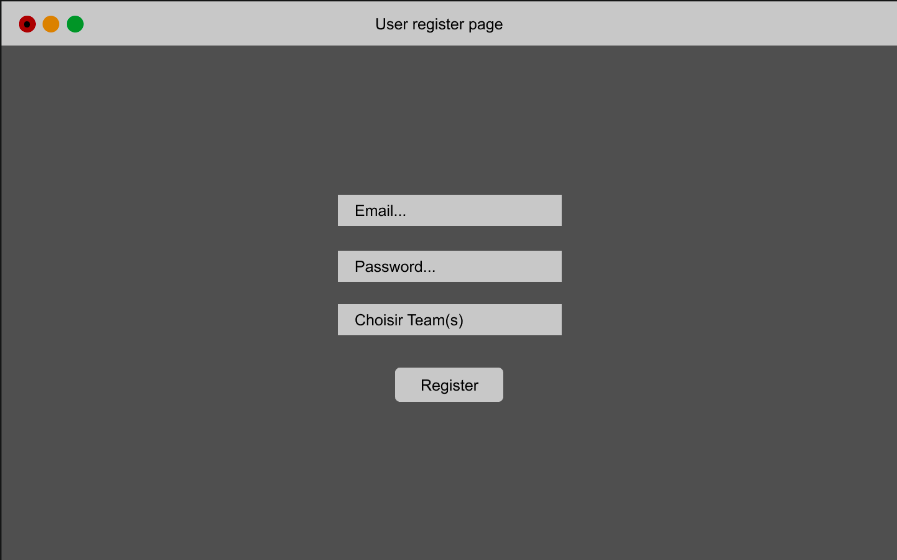
\includegraphics[scale=0.3]{mockup/m_user_register}
		\caption{Interface d'ajout de nouveaux utilisateurs}
		\label{fig:userRegister}
	\end{figure}
	
	Cette page en Figure ~\ref{fig:userRegister} servira de page d'ajout d'utilisateur et sera accessible par tous (dans le cadre de mon TB en tout cas).
		
	\begin{figure}[h!]
		\centering
		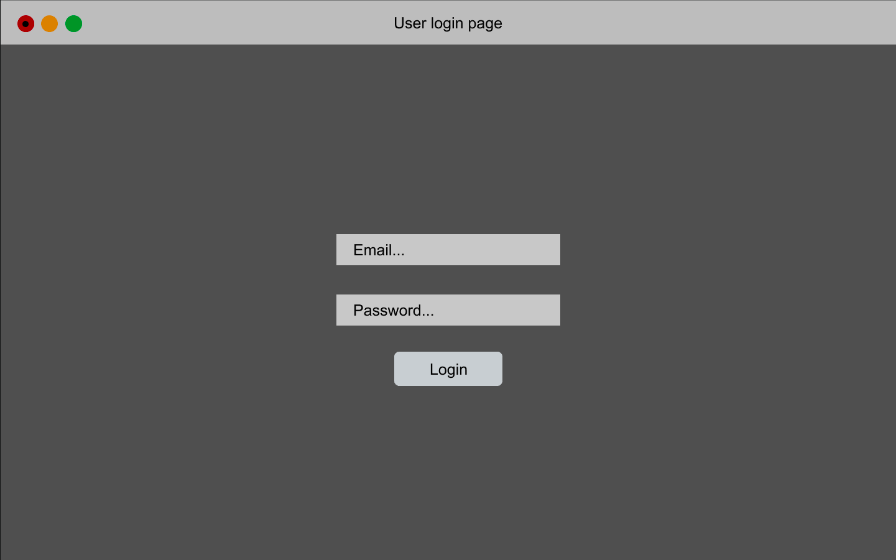
\includegraphics[scale=0.3]{mockup/m_user_login}
		\caption{Interface de connexion des utilisateurs}
		\label{fig:userLogin}
	\end{figure}
	
	La page de login est simple et standard.
	
\newpage
\subsection{Ecrans}
	
	\begin{figure}[h]
		\centering
		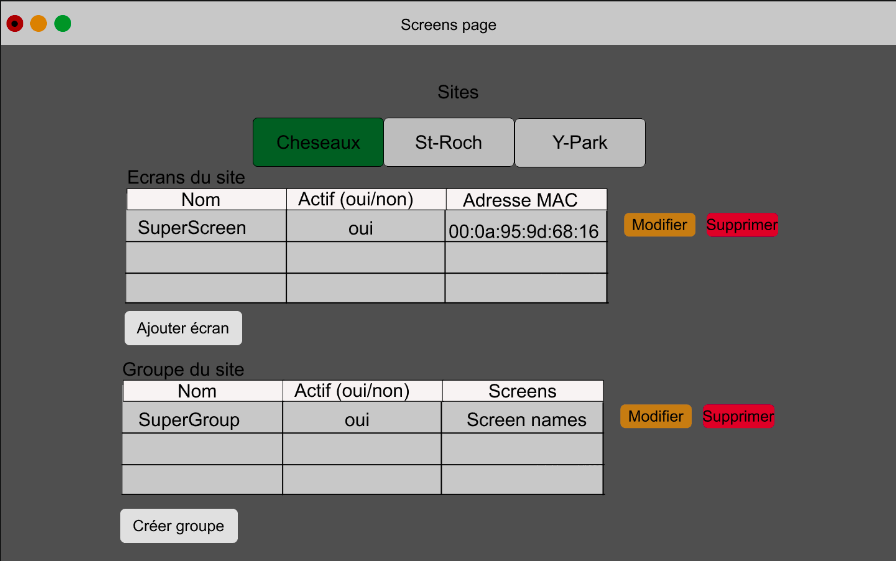
\includegraphics[scale=0.3]{mockup/m_screens_page}
		\caption{Page principale des écrans}
		\label{fig:screenPage}
	\end{figure}
	
	Cette page affichera les écrans accessibles par l'utilisateur actuel, regroupés par site. On aura également accès aux groupes d'écrans. C'est depuis cette page qu'on pourra rajouter des écrans.
	
	\begin{figure}[h]
		\centering
		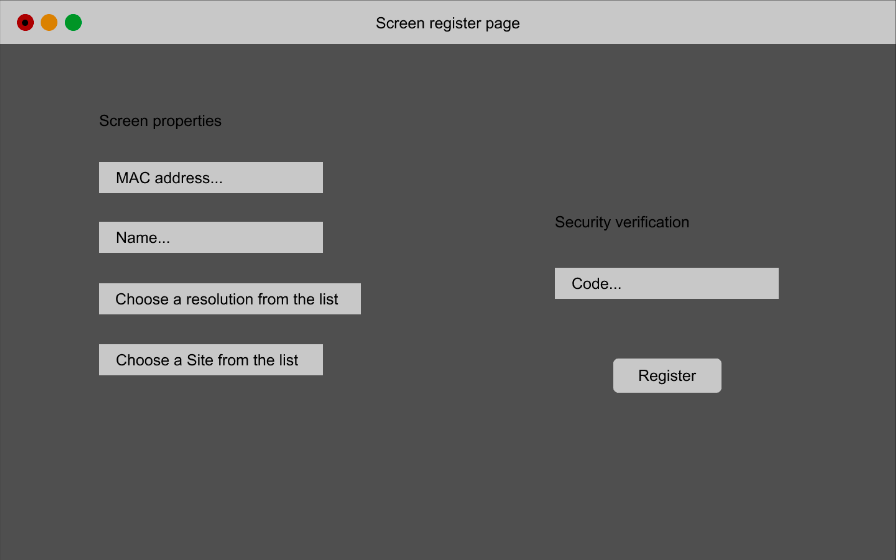
\includegraphics[scale=0.3]{mockup/m_screen_register}
		\caption{Interface d'ajout de nouvel écran}
		\label{fig:screenRegister}
	\end{figure}
	
	L'administrateur peut ajouter un nouvel écran au système par le biais de cette interface. Il doit préciser quelques paramètres et surtout donner le code fourni précédemment par le serveur.
	
\newpage
\subsection{Teams}

	\begin{figure}[ht!]
		\centering
		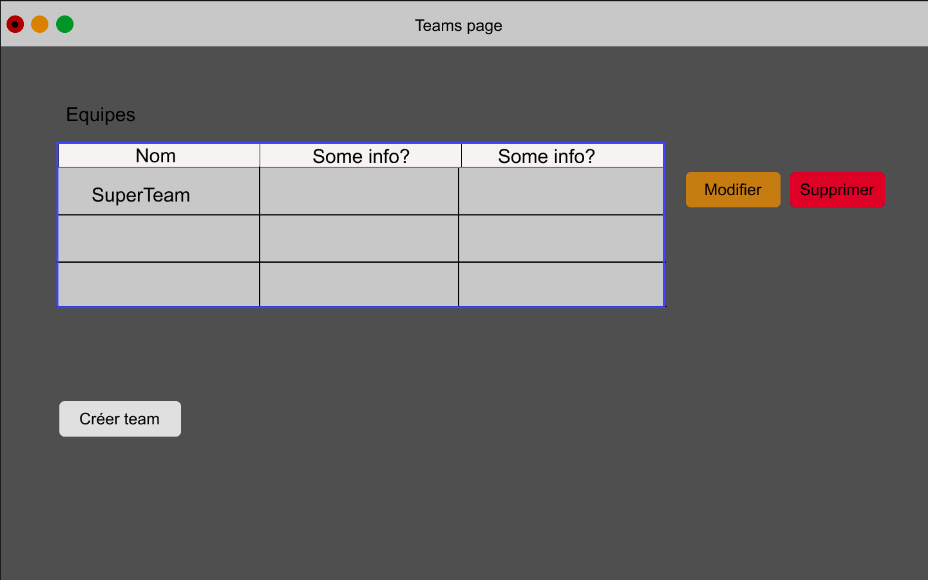
\includegraphics[scale=0.3]{mockup/m_teams_page}
		\caption{Page principale des teams}
		\label{fig:teamPage}
	\end{figure}
	
	Cette page sera accessible uniquement par les administrateurs car elle répertoriera les différentes Team de l'application avec la possibilité d'effectuer des actions dessus.
	
	\begin{figure}[h]
		\centering
		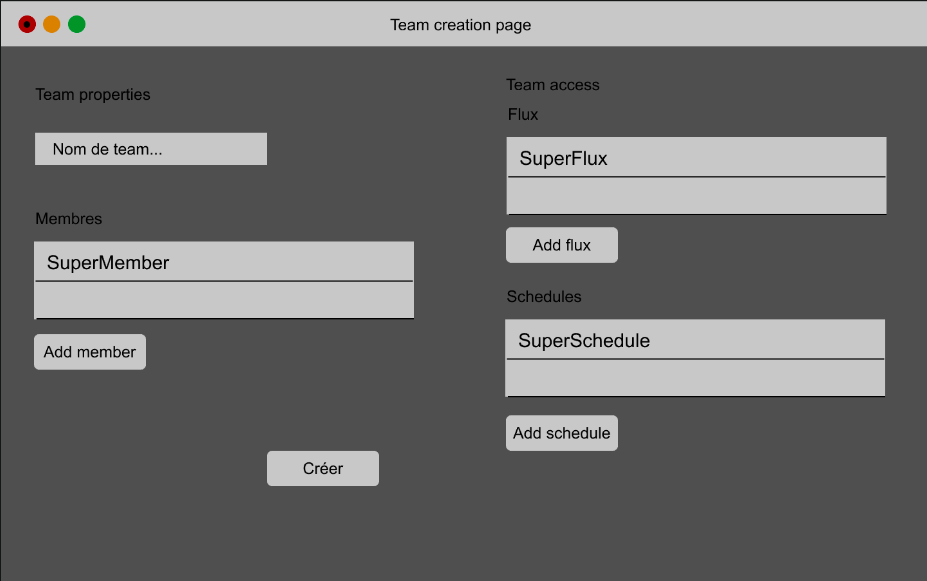
\includegraphics[scale=0.3]{mockup/m_team_creation}
		\caption{Interface de création de team}
		\label{fig:teamCreation}
	\end{figure}
	
	On pourra créer des Team en spécifiant directement les objets auxquels elle a accès (Flux, Schedules, Membres, etc).

\newpage	
\subsection{Flux}

	\begin{figure}[h]
		\centering
		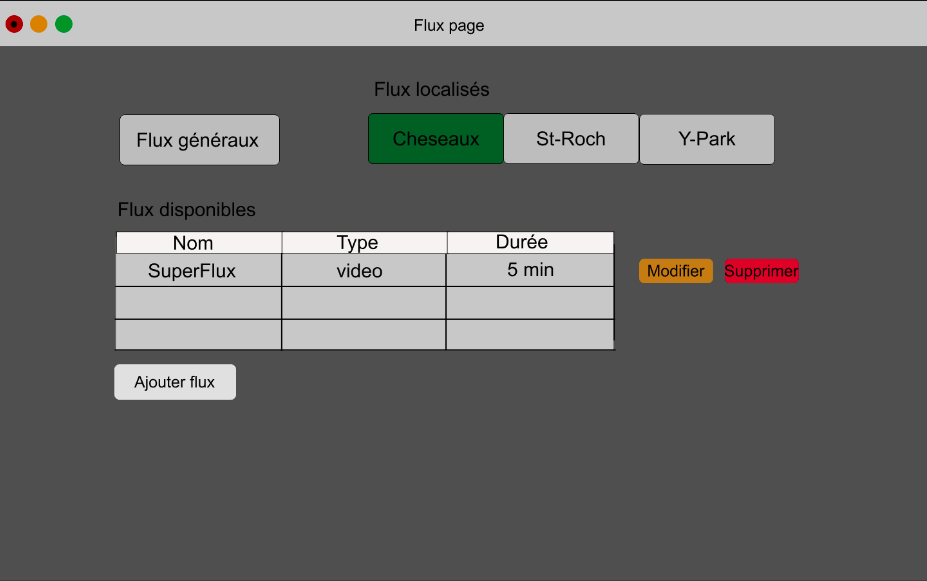
\includegraphics[scale=0.3]{mockup/m_flux_page}
		\caption{Page principale des flux}
		\label{fig:fluxPage}
	\end{figure}
	
	
	Cette page affichera les flux disponibles pour la Team courante et permettra également des opérations sur ces flux. Idéalement, ils seraient regroupés par site.
	
	\begin{figure}[h]
		\centering
		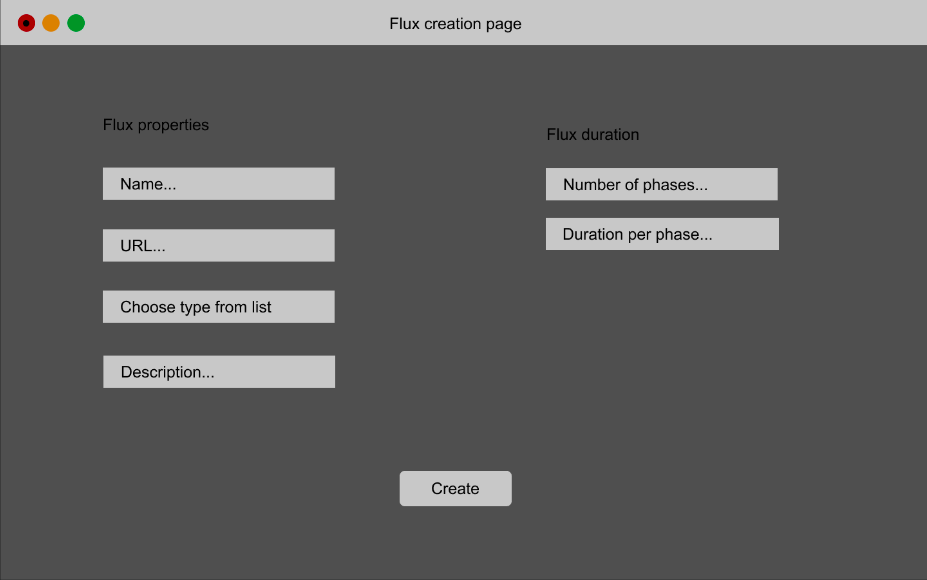
\includegraphics[scale=0.3]{mockup/m_flux_creation}
		\caption{Interface de création de flux}
		\label{fig:fluxCreation}
	\end{figure}
	
	C'est depuis cette page que l'on pourra créer de nouveaux flux.
	
\newpage
\subsection{Schedules}

	\begin{figure}[h]
		\centering
		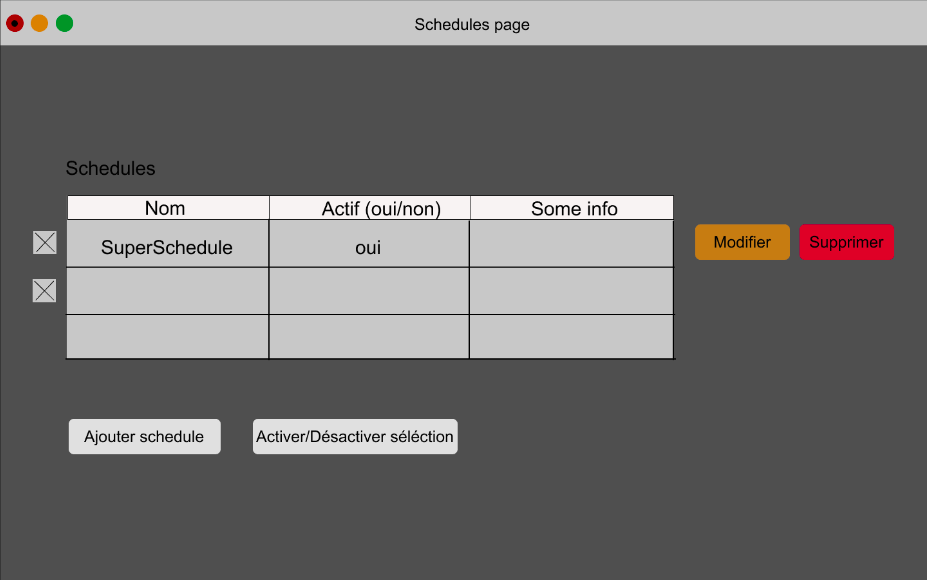
\includegraphics[scale=0.3]{mockup/m_schedules_page}
		\caption{Page principale des Schedules}
		\label{fig:schedulePage}
	\end{figure}
	Cette page affichera les Schedules de la Team courante et permettra des les activer/désactiver en plus des actions standards.
	
	\begin{figure}[h]
		\centering
		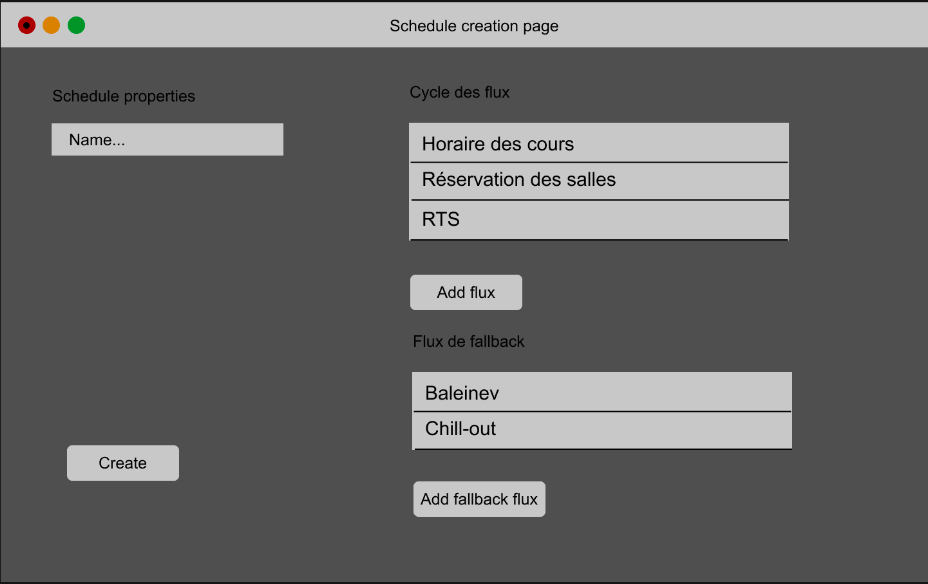
\includegraphics[scale=0.3]{mockup/m_schedule_creation}
		\caption{Interface de création de Schedule}
		\label{fig:scheduleCreation}
	\end{figure}
	
	On choisit les flux qui vont constituer le cycle du Schedule. On peut également définir des flux de fallback qui prendront le relai si le flux actif n'a aucune information à afficher.

\newpage
\subsection{Diffusers}

	\begin{figure}[h]
		\centering
		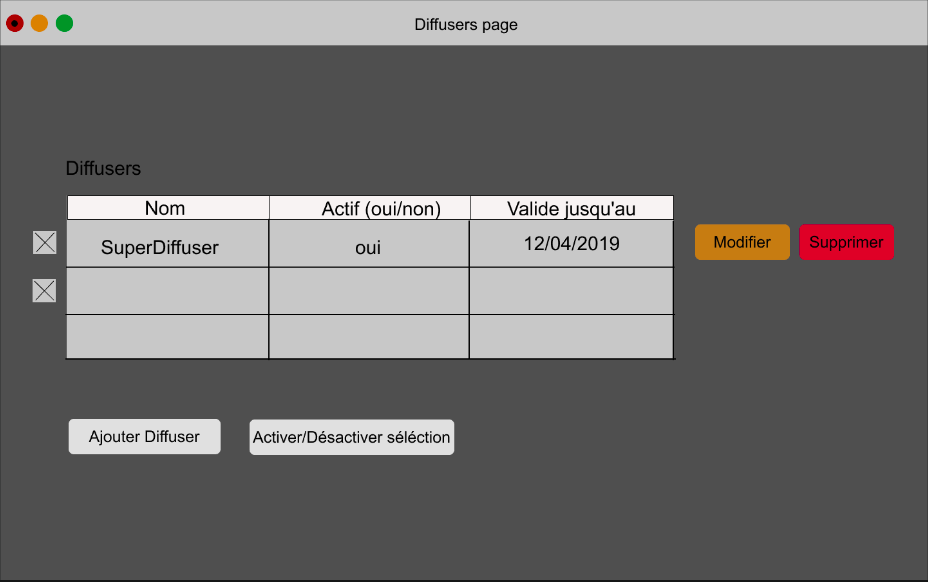
\includegraphics[scale=0.3]{mockup/m_diffusers_page}
		\caption{Page principale des diffusers}
		\label{fig:diffuserPage}
	\end{figure}
	
	Comme pour les Schedules, cette page permet d'activer/désactiver des Diffusers en plus des actions standards.
	
	\begin{figure}[h!]
		\centering
		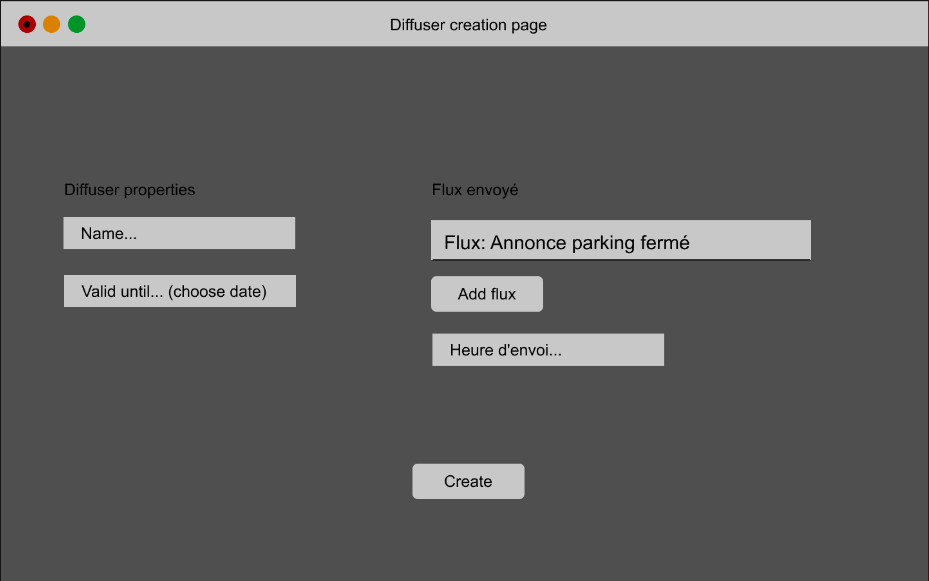
\includegraphics[scale=0.3]{mockup/m_diffuser_creation}
		\caption{Interface de création de diffuser}
		\label{fig:diffuserCreation}
	\end{figure}
	
	On crée un Diffuser en choisissant une heure de début, un flux et une durée de validité.
 
\end{appendices}

\newpage
\begin{thebibliography}{9}
\bibitem{playdoc} 
Play Framwork documentation:
\\\texttt{https://www.playframework.com/documentation/2.7.x/Home}
 
\bibitem{eventsourcegit} 
Exemple de solution SSE avec Scala Play:
\\\texttt{https://github.com/septeni-original/play-scala-sse-example}

\bibitem{stackoverflow} 
Stack Overflow, pour des réponses à mes questions:
\\\texttt{https://stackoverflow.com/}

\bibitem{bootstraptable}
Exemple de table Bootstrap dynamique:
\\\texttt{https://www.tutorialrepublic.com/snippets/preview.php?topic=bootstrap\&file=table-with-add-and-delete-row-feature}

\bibitem{mozillaeventsource}
Documentation sur les Eventsource:
\\\texttt{https://developer.mozilla.org/en-US/docs/Web/API/EventSource}
\\\texttt{https://developer.mozilla.org/en-US/docs/Web/API/Server-sent\_events/Using\_server-sent\_events}

\bibitem{quartz} 
Documentation de Quartz: 
\\\texttt{http://www.quartz-scheduler.org/documentation/}


\end{thebibliography}

\end{document}
















